%%%%%%%%%%%%%%%%%%%%%%%%%%%%%%%%%%%%%%%%%%%%%%%%%%%%%%%%%%%%%%%%%%%%%%
%     File: ExtendedAbstract_resul.tex                               %
%     Tex Master: ExtendedAbstract.tex                               %
%                                                                    %
%     Author: Andre Calado Marta                                     %
%     Last modified : 27 Dez 2011                                    %
%%%%%%%%%%%%%%%%%%%%%%%%%%%%%%%%%%%%%%%%%%%%%%%%%%%%%%%%%%%%%%%%%%%%%%
% Results
% Results should be clear and concise.
% Discussion
% This should explore the significance of the results of the work, not
% repeat them. A combined Results and Discussion section is often
% appropriate. Avoid extensive citations and discussion of published
% literature.
%%%%%%%%%%%%%%%%%%%%%%%%%%%%%%%%%%%%%%%%%%%%%%%%%%%%%%%%%%%%%%%%%%%%%%

\section{Results}
\label{sec:resul}

\begin{figure}[H]
  \centering
  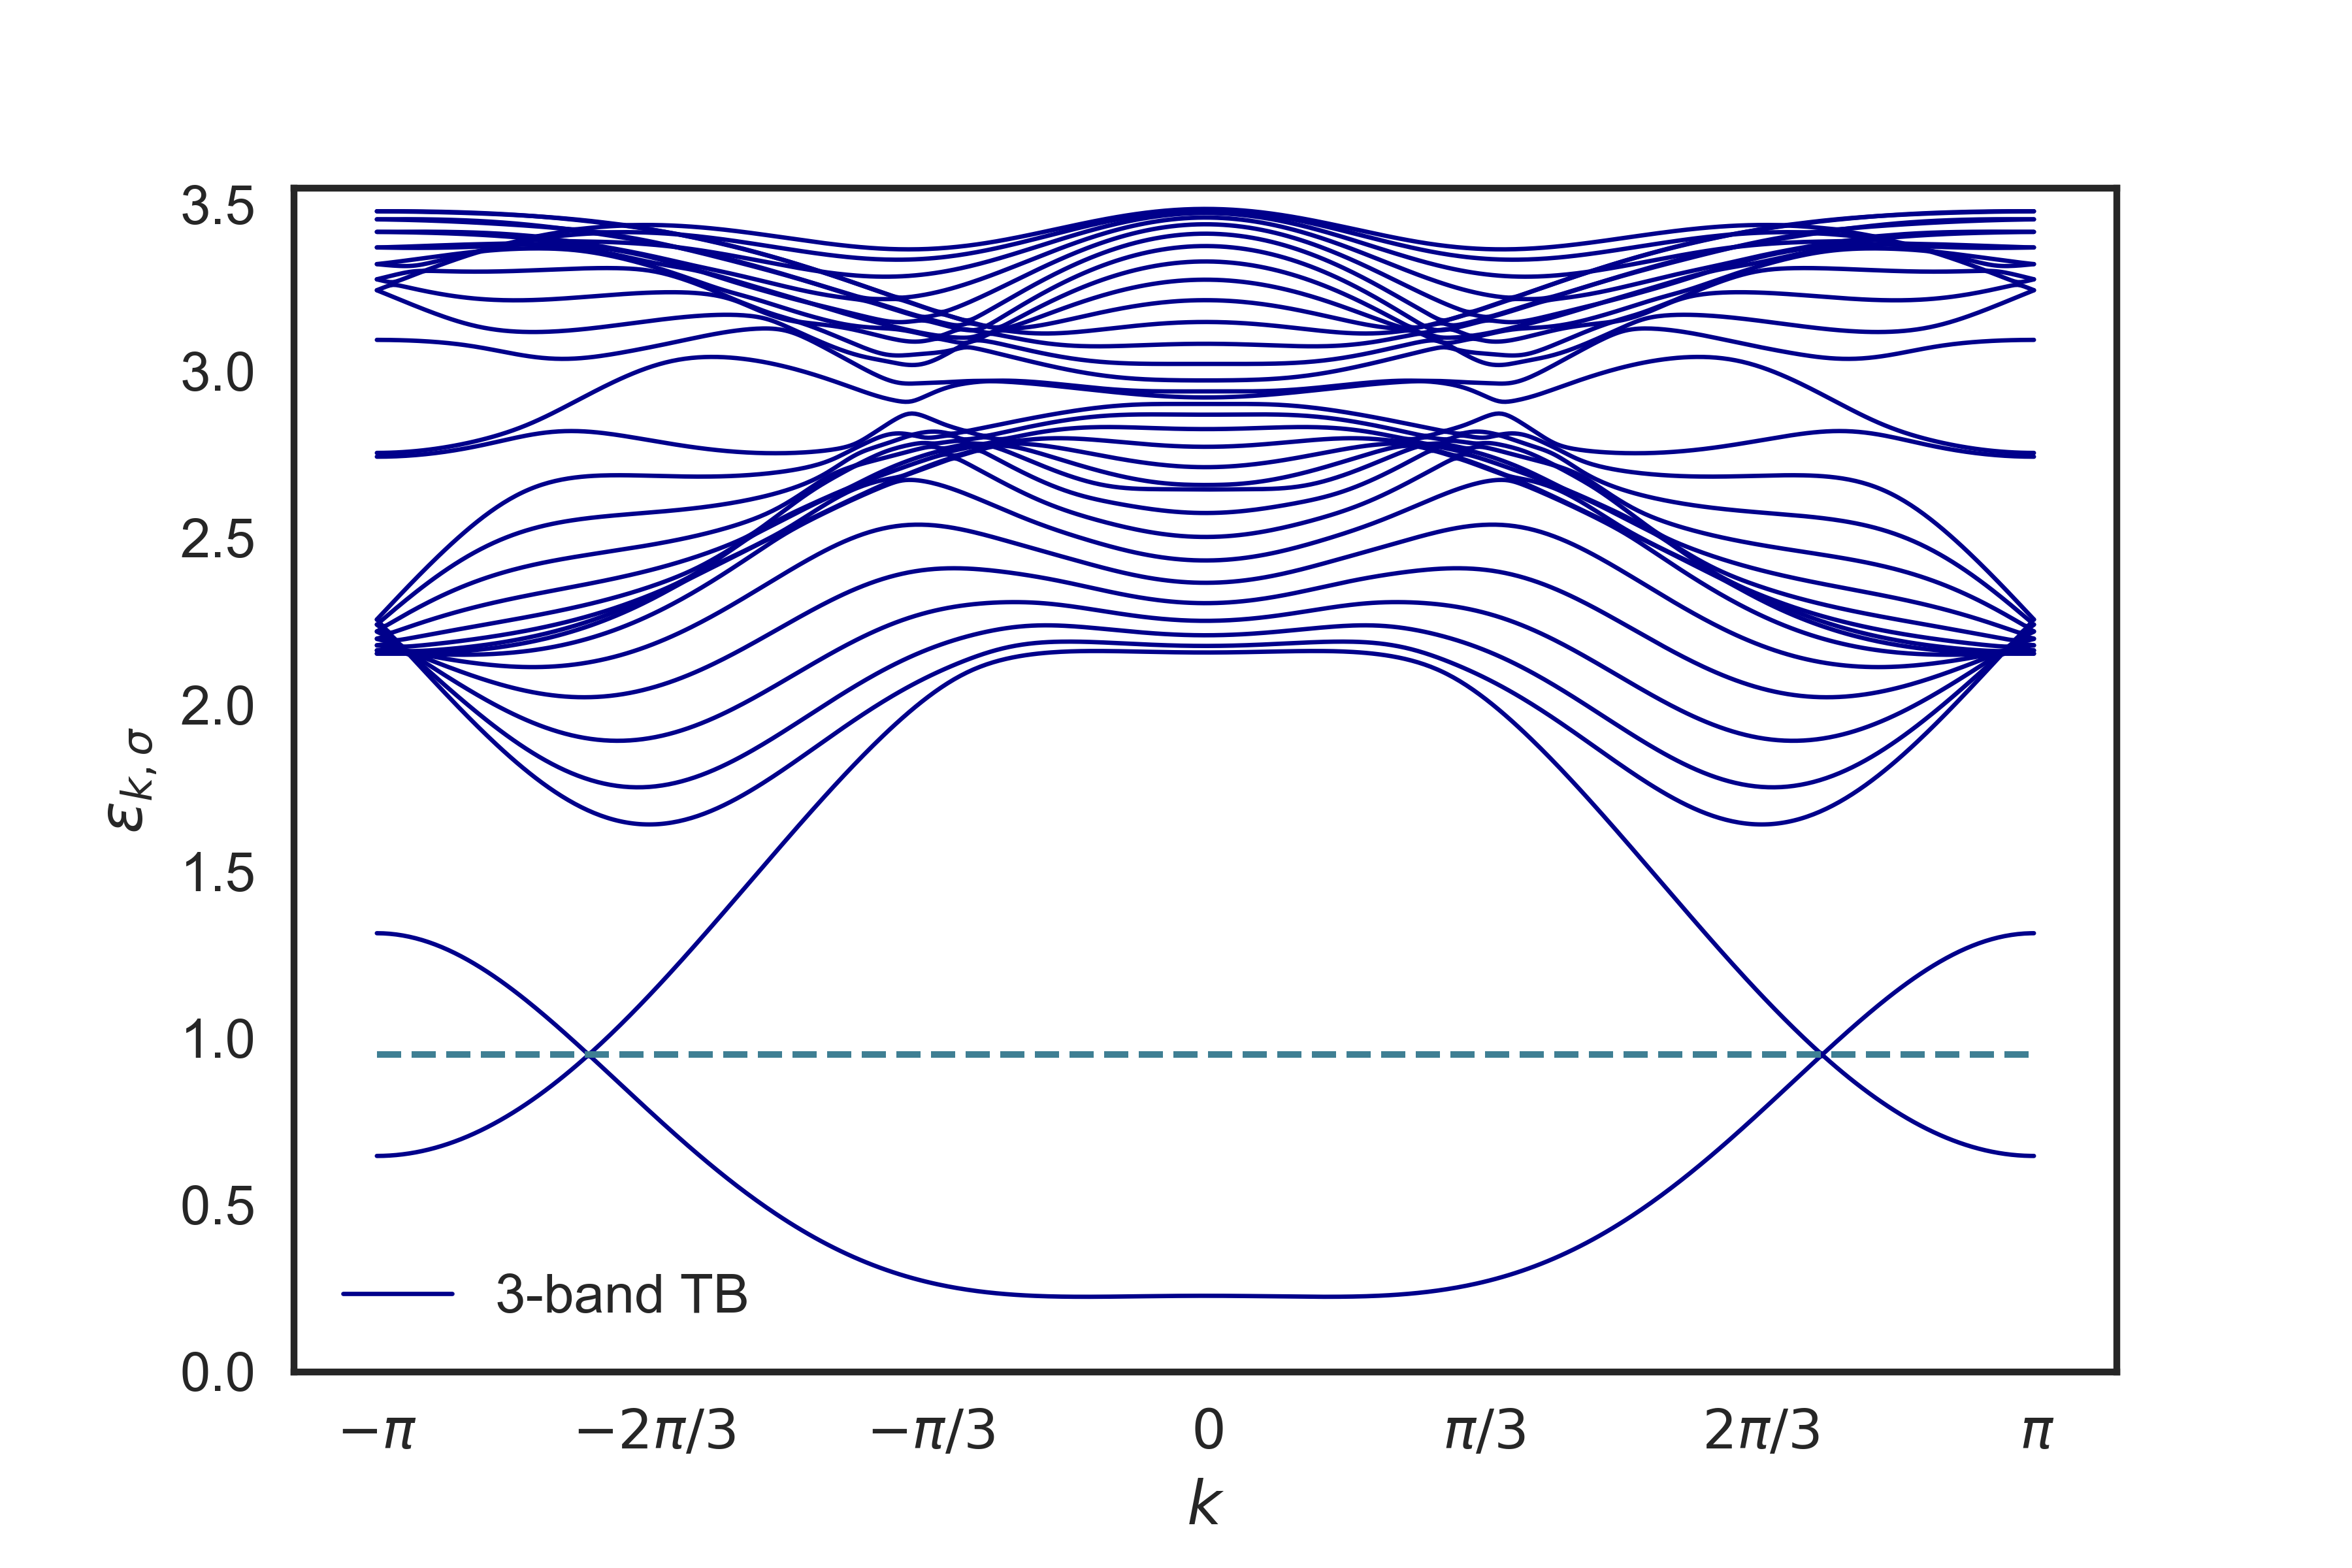
\includegraphics[width=6cm]{images/freeBands.png}
  \caption{Comparison with \texttt{QUEST}}
  \label{fig:blade_flow_pressure}
\end{figure}

\begin{figure}[H]
  \centering
  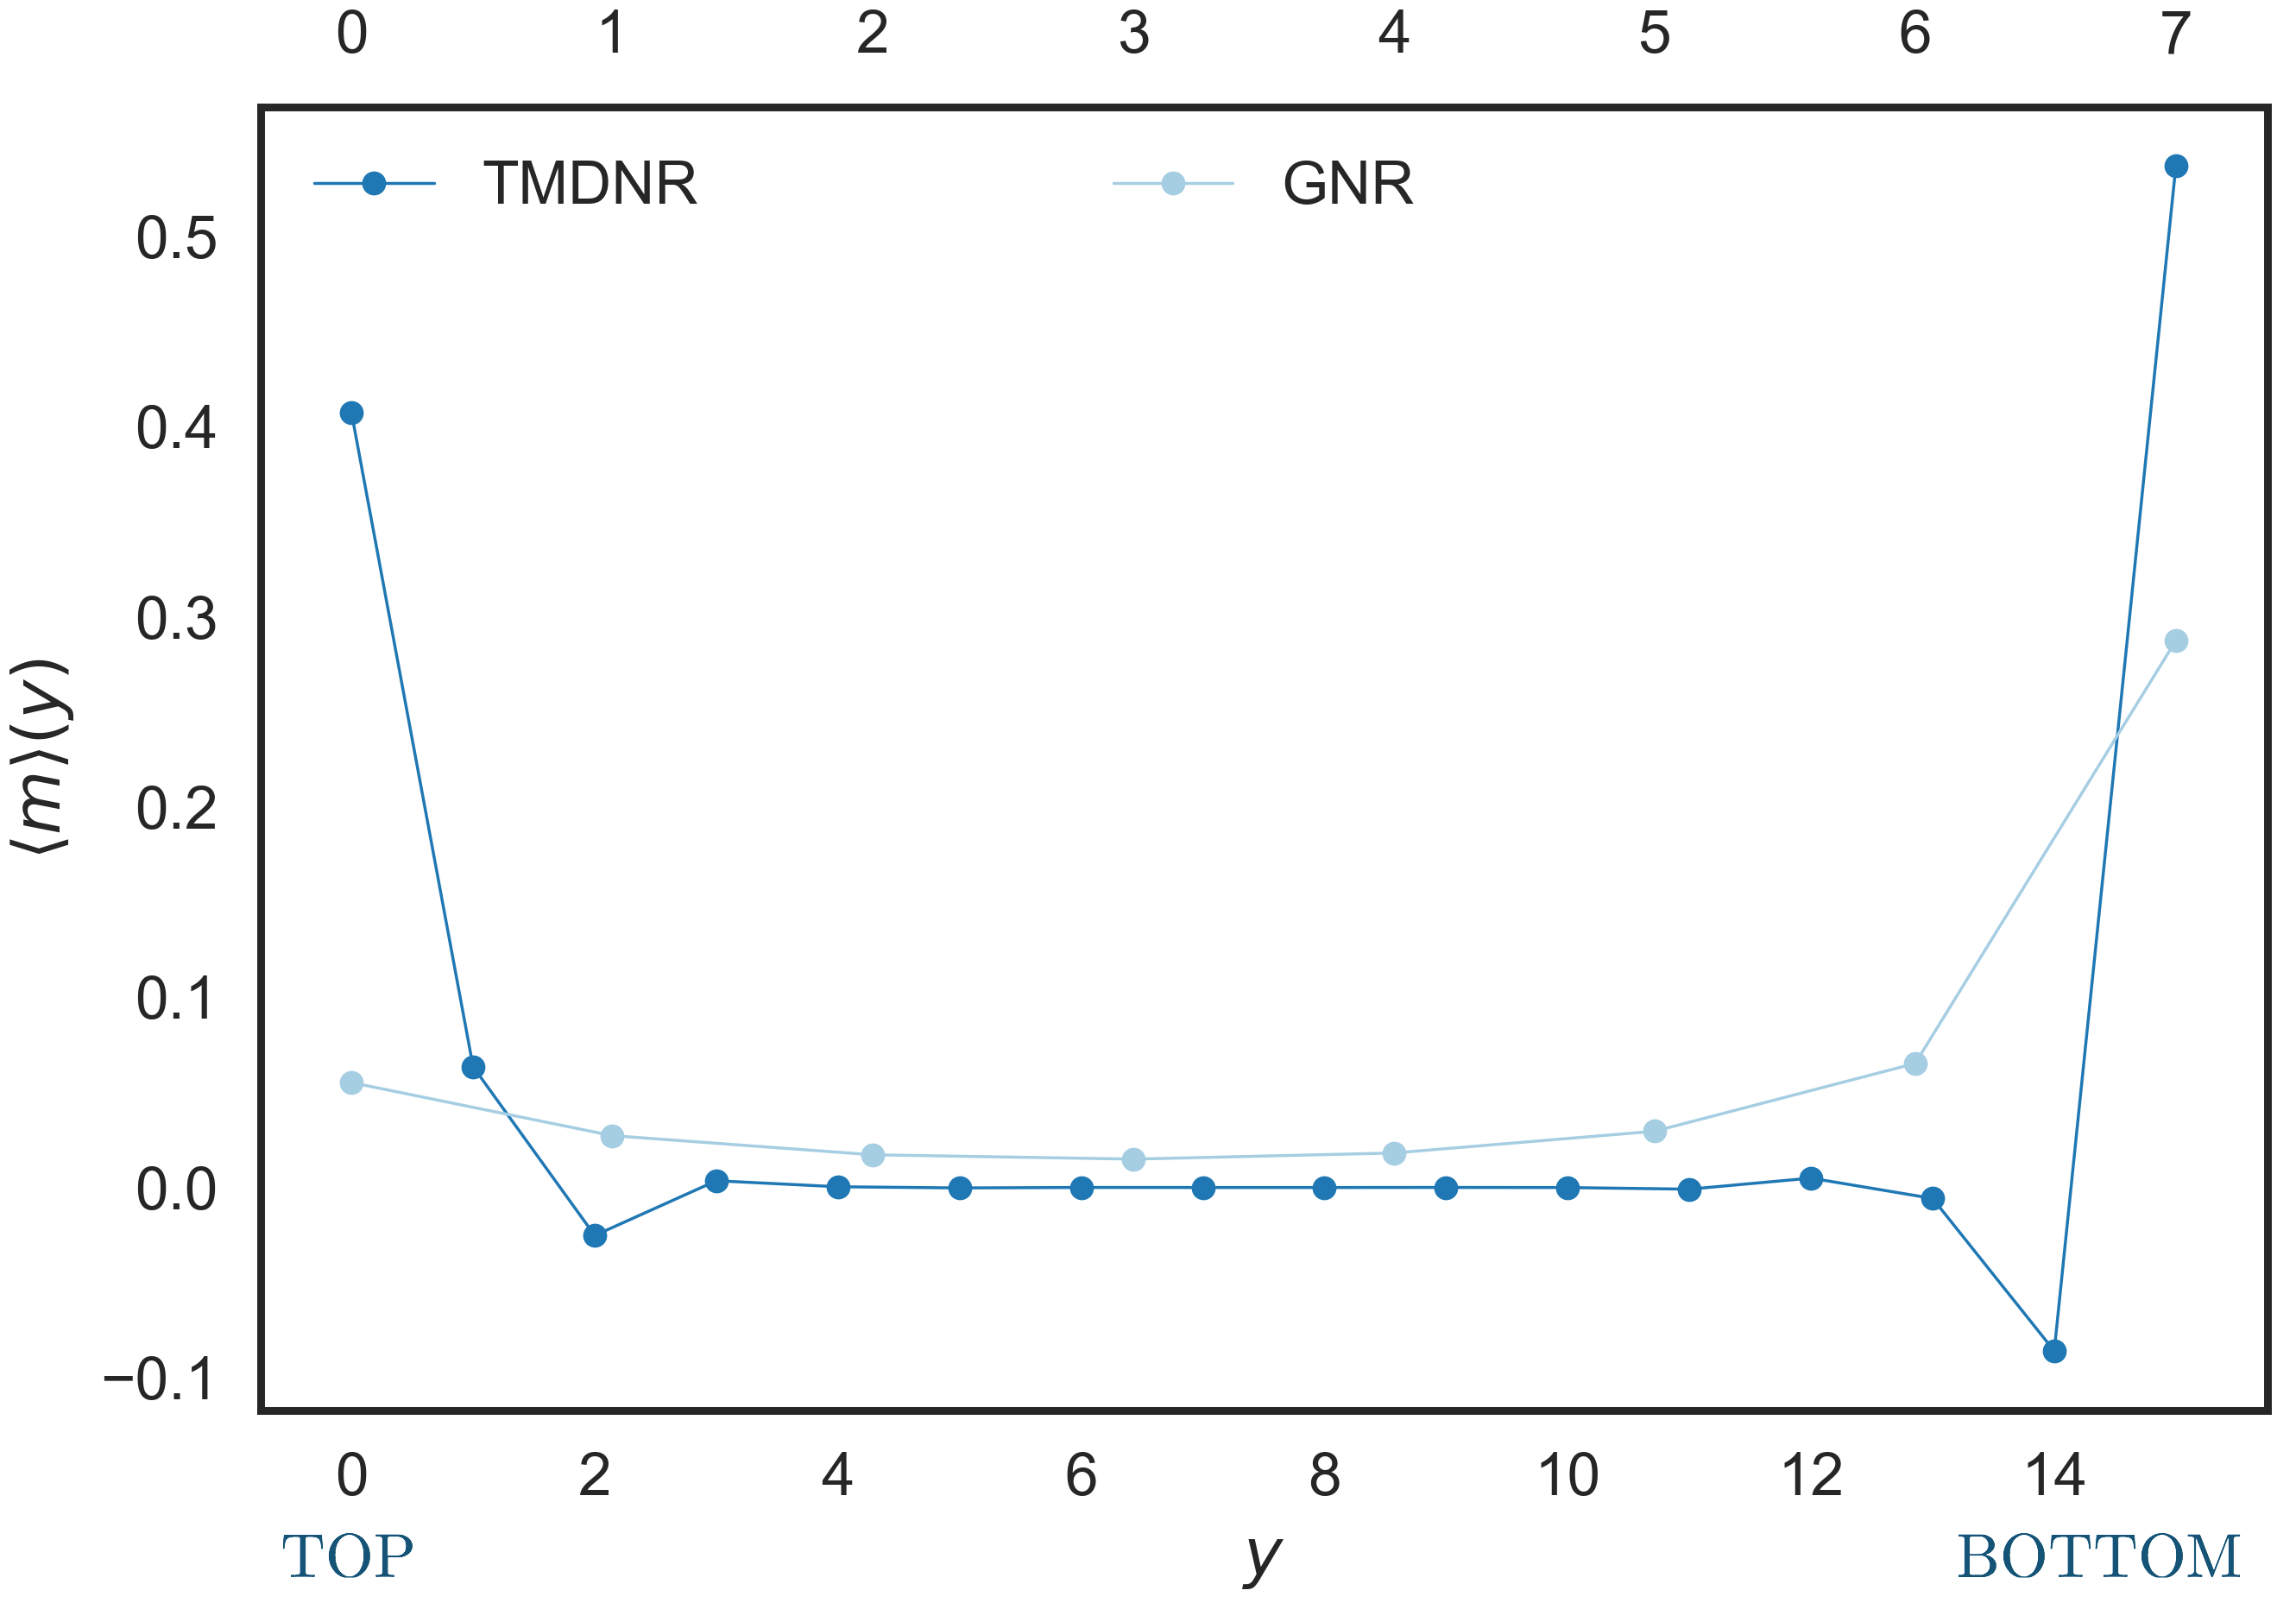
\includegraphics[width=6cm]{images/magProf.png}
  \caption{Comparison with \texttt{QUEST}}
  \label{fig:blade_flow_pressure}
\end{figure}

\begin{figure}[H]
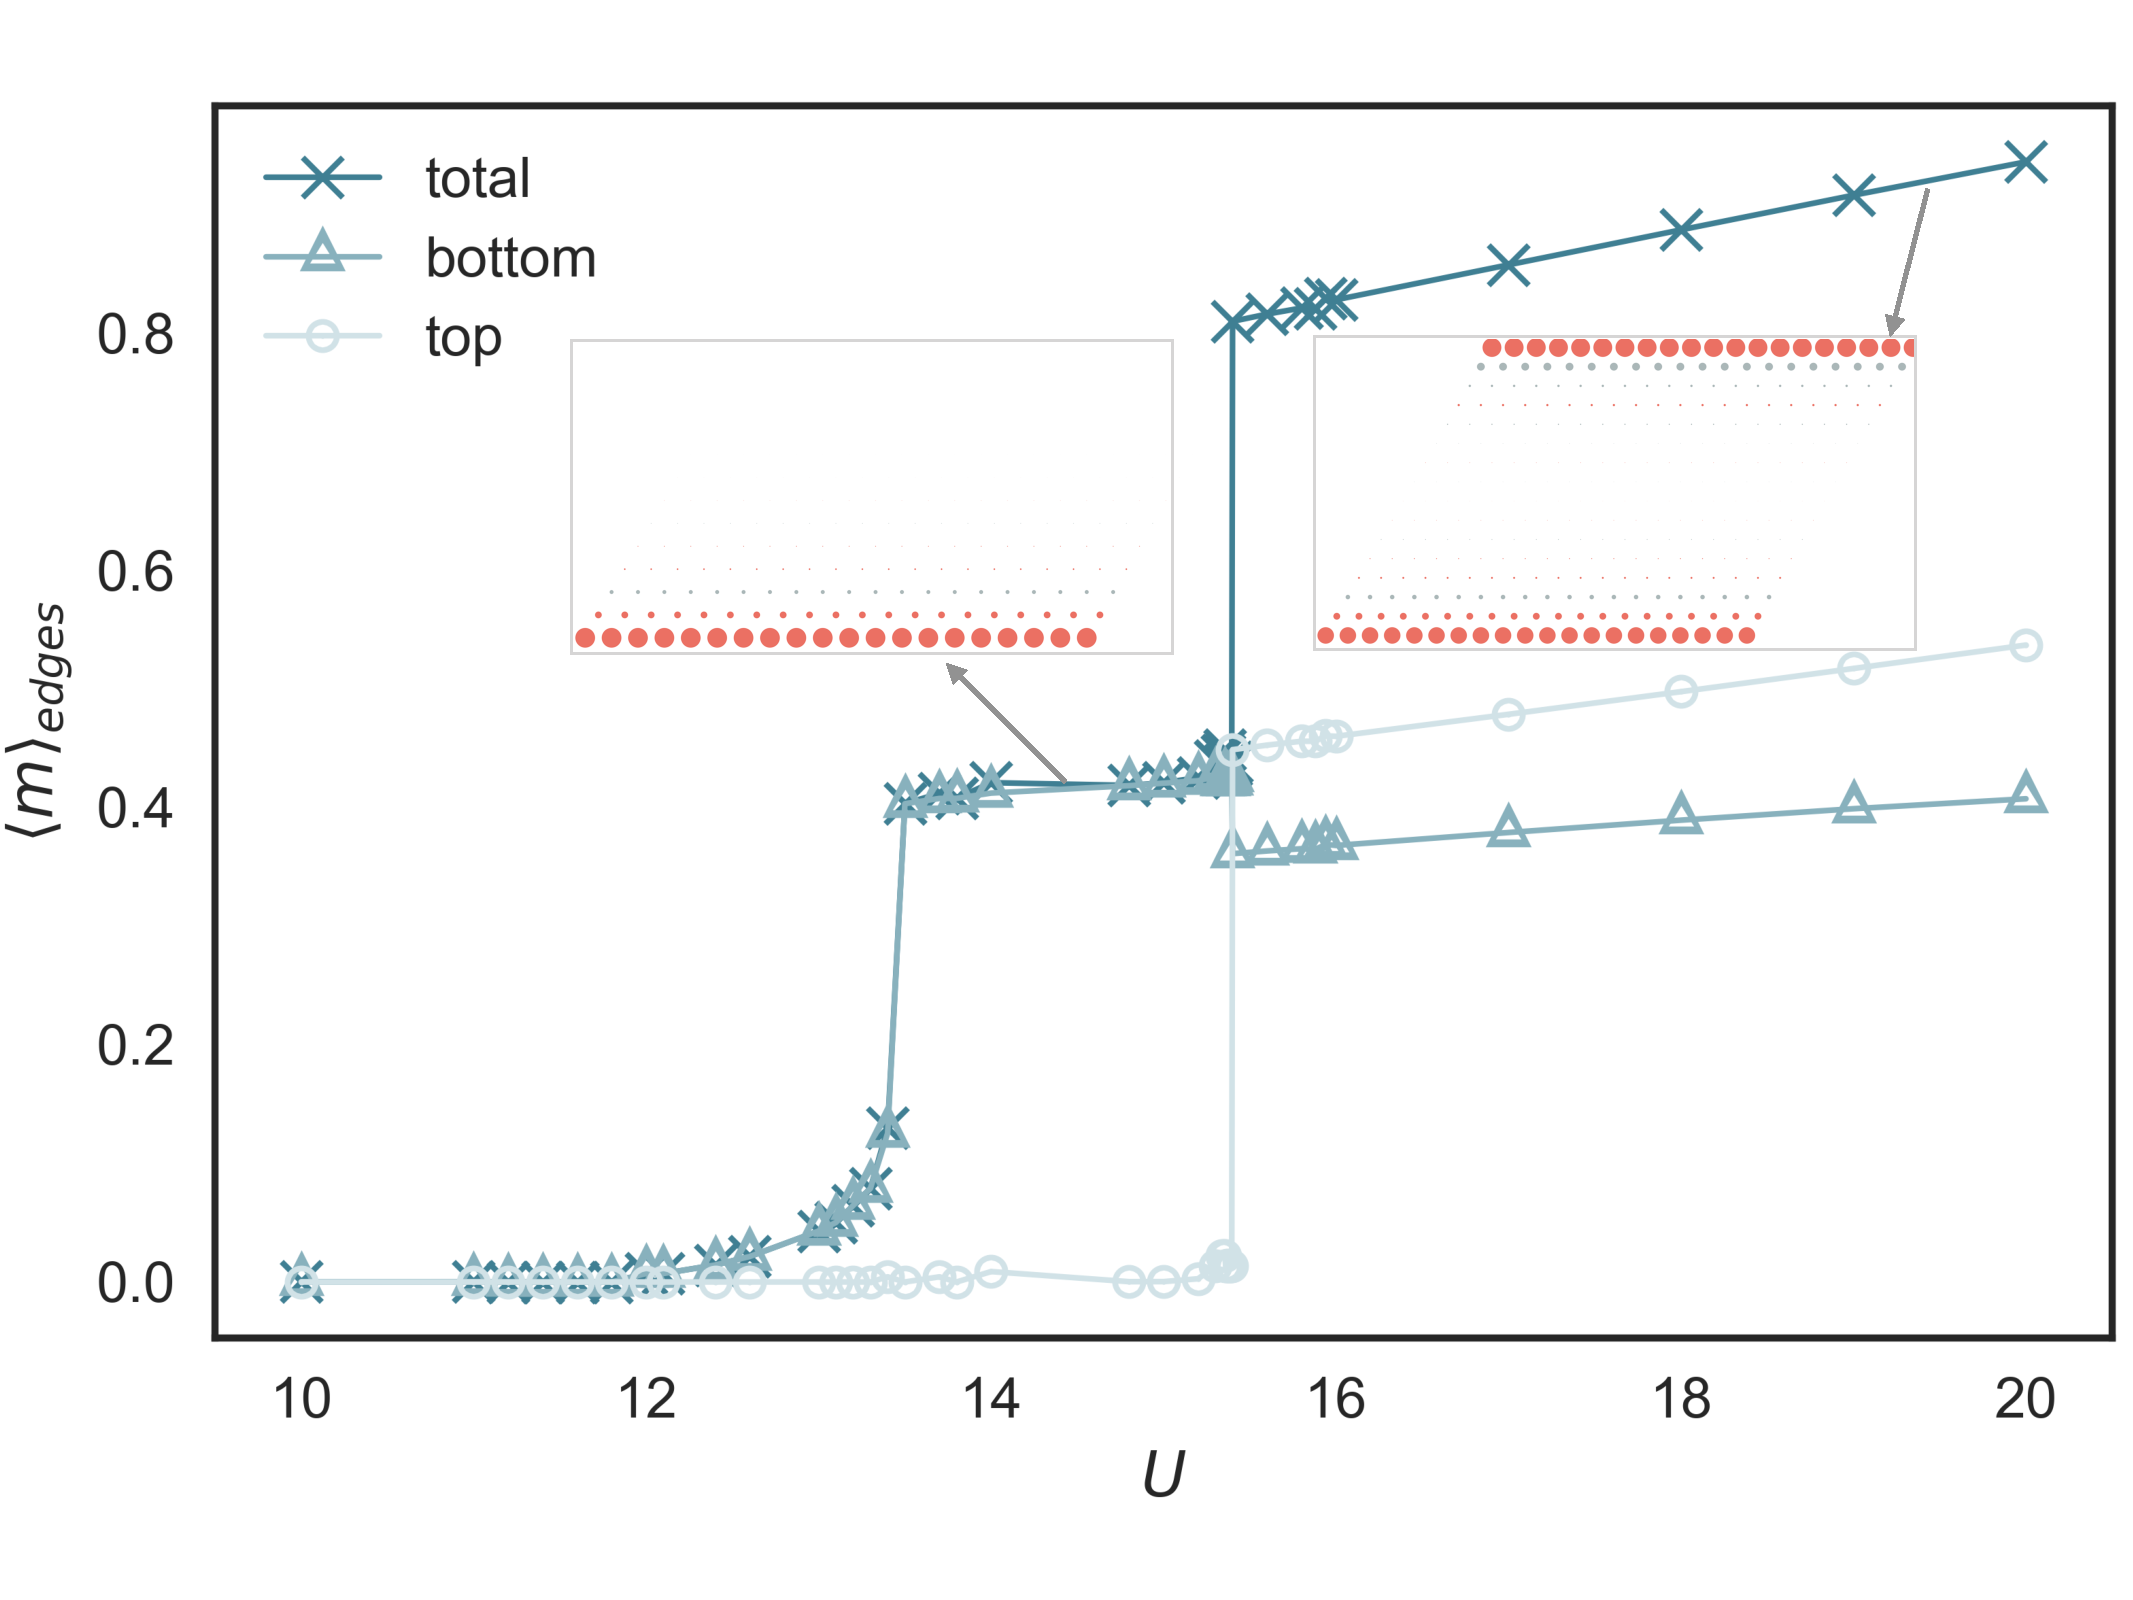
\includegraphics[trim={0cm 1.7cm 0cm 1.7cm},clip, scale =0.21]{images/edge-mag.pdf}
	\caption[Mean field phase diagram at zero temperature. Zoom-in of the first phase transition.]{Mean field phase diagram at zero temperature. Zoom-in of the first phase transition.
	\label{fig:zeroTphaseDiagram}}
\end{figure}

\begin{figure}[H]
\centering
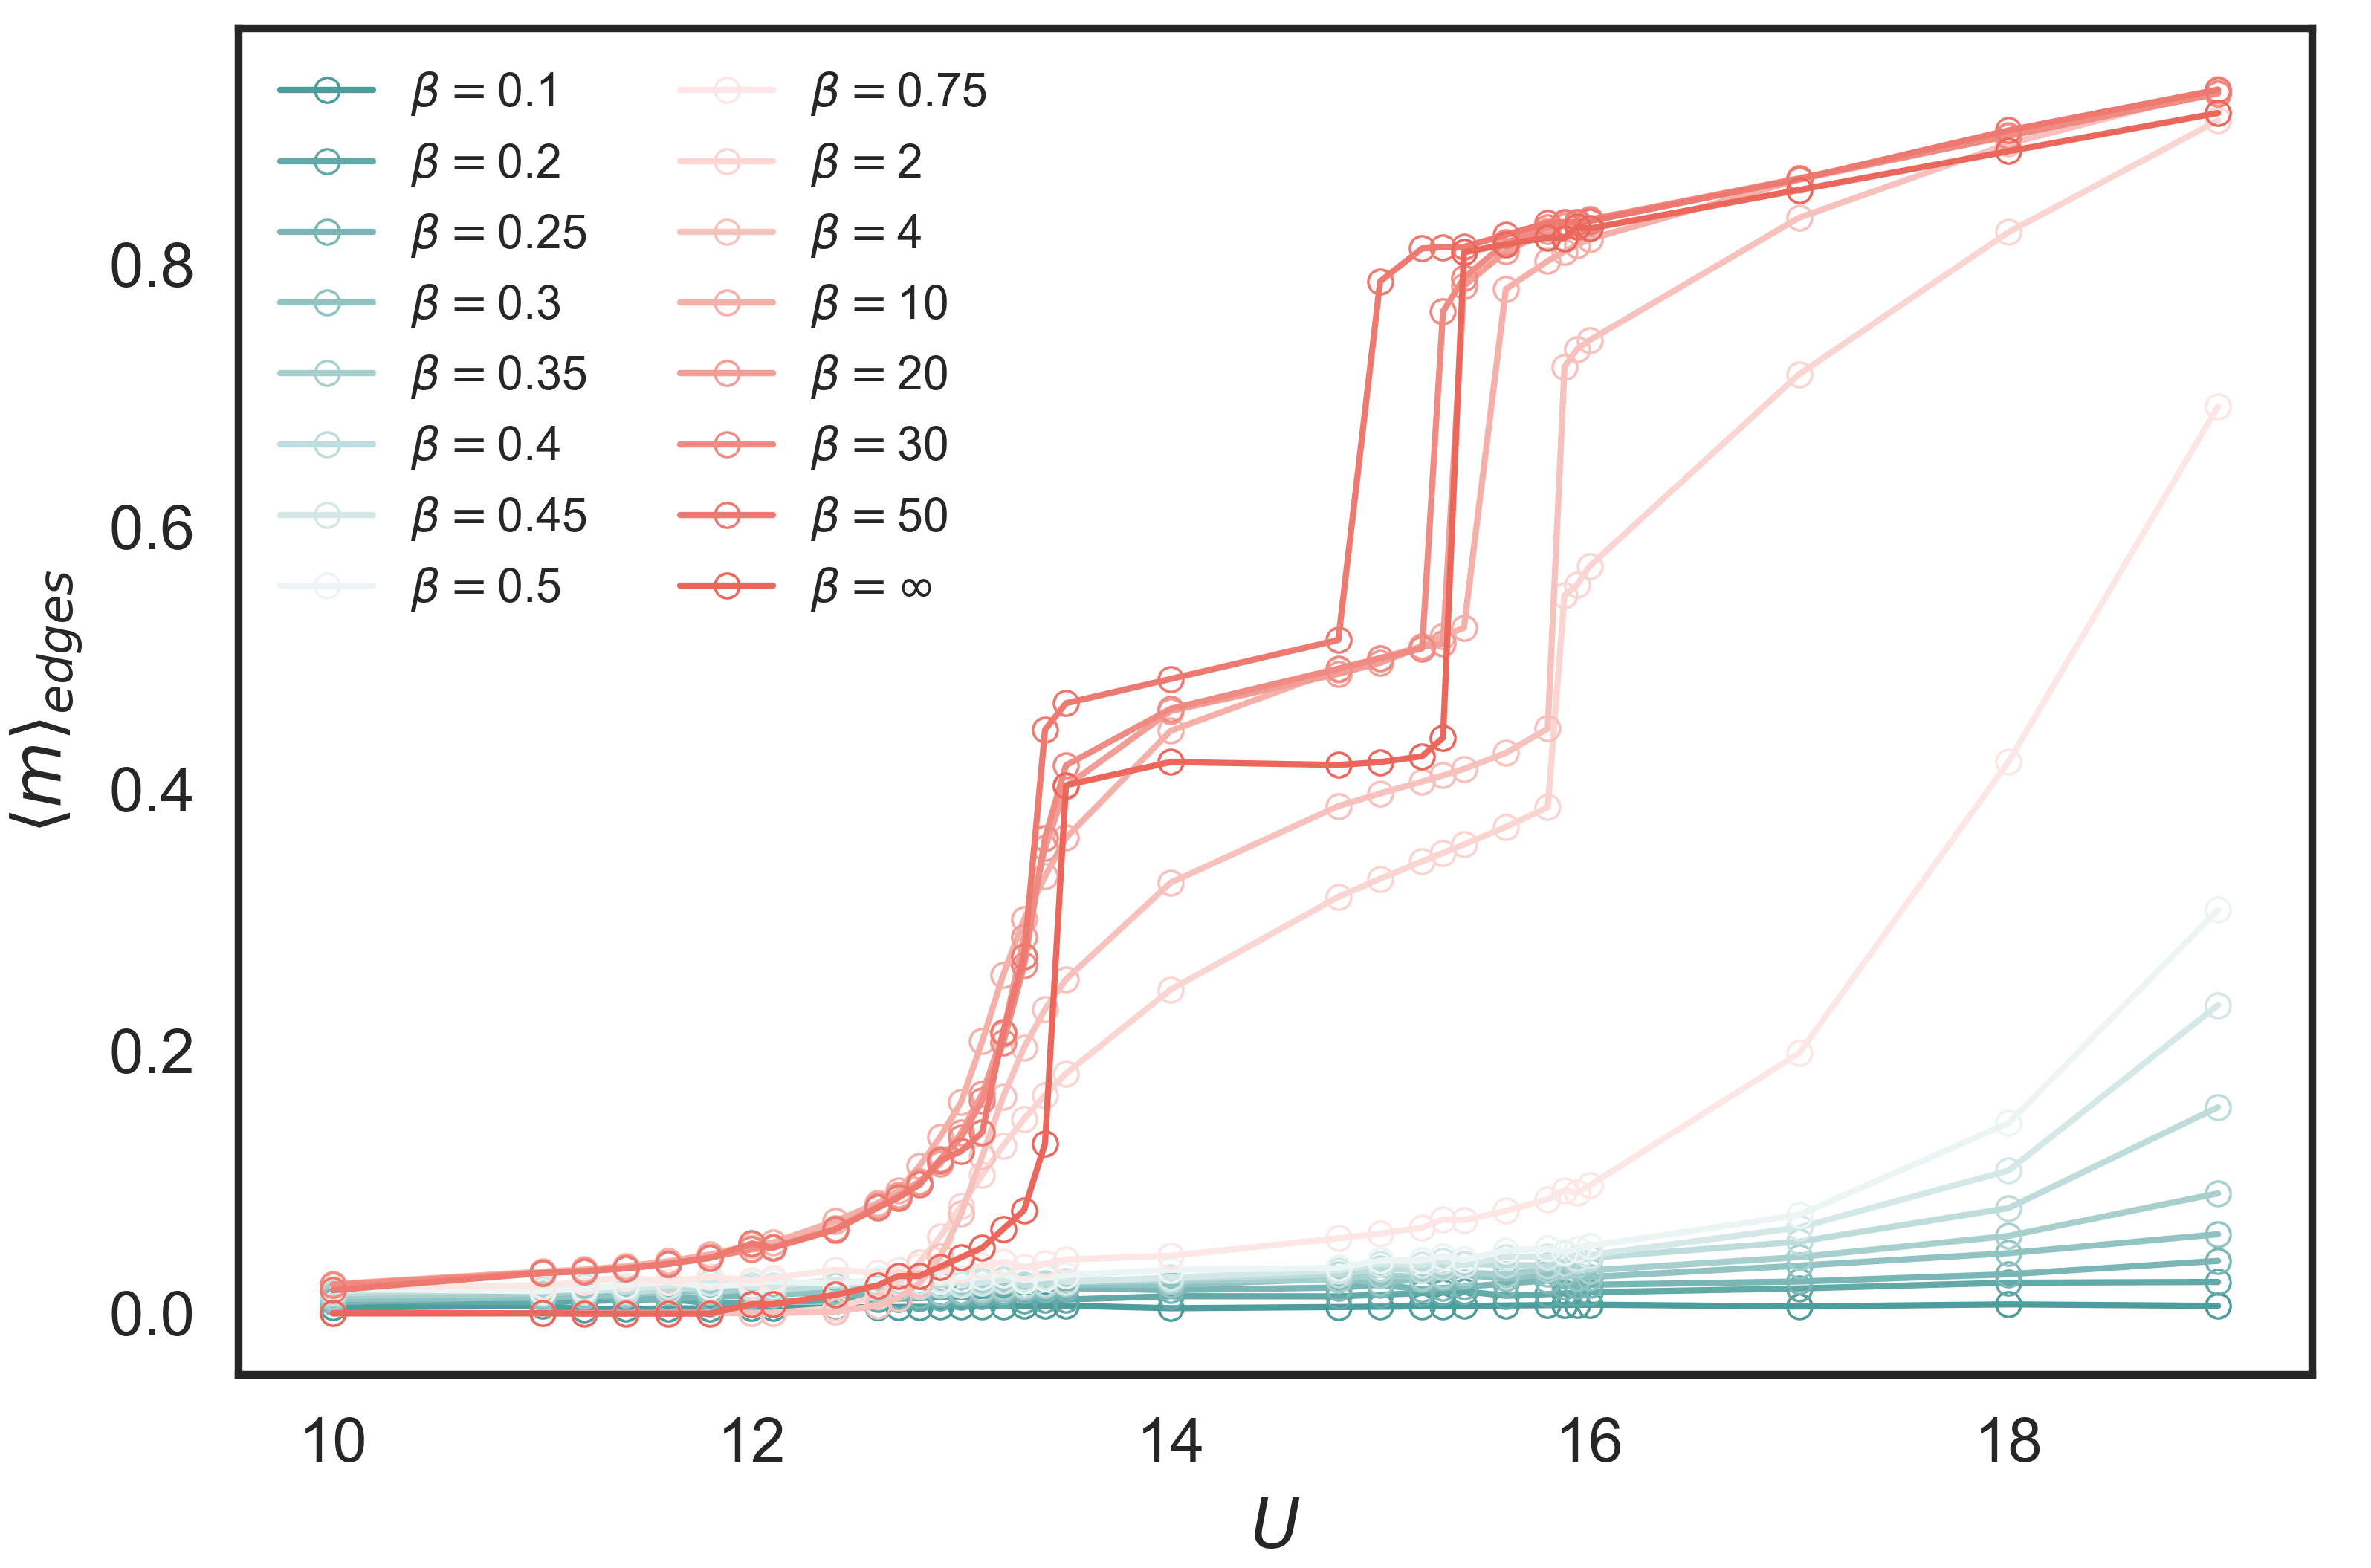
\includegraphics[scale =0.5]{images/edge-mag-phase-diagram.png}
	\caption[$T=0$ mean field band structure for a TMD nanoribbon of width $N_y = 16$ in the ordered phase, at $U=20 | t_0 |$.]{$T=0$ mean field band structure for a TMD nanoribbon of width $N_y = 16$ in the ordered phase ($U=20 | t_0 |$).}
	\label{fig:bandsZoomed}
\end{figure}

\begin{figure}[H]
  \centering
  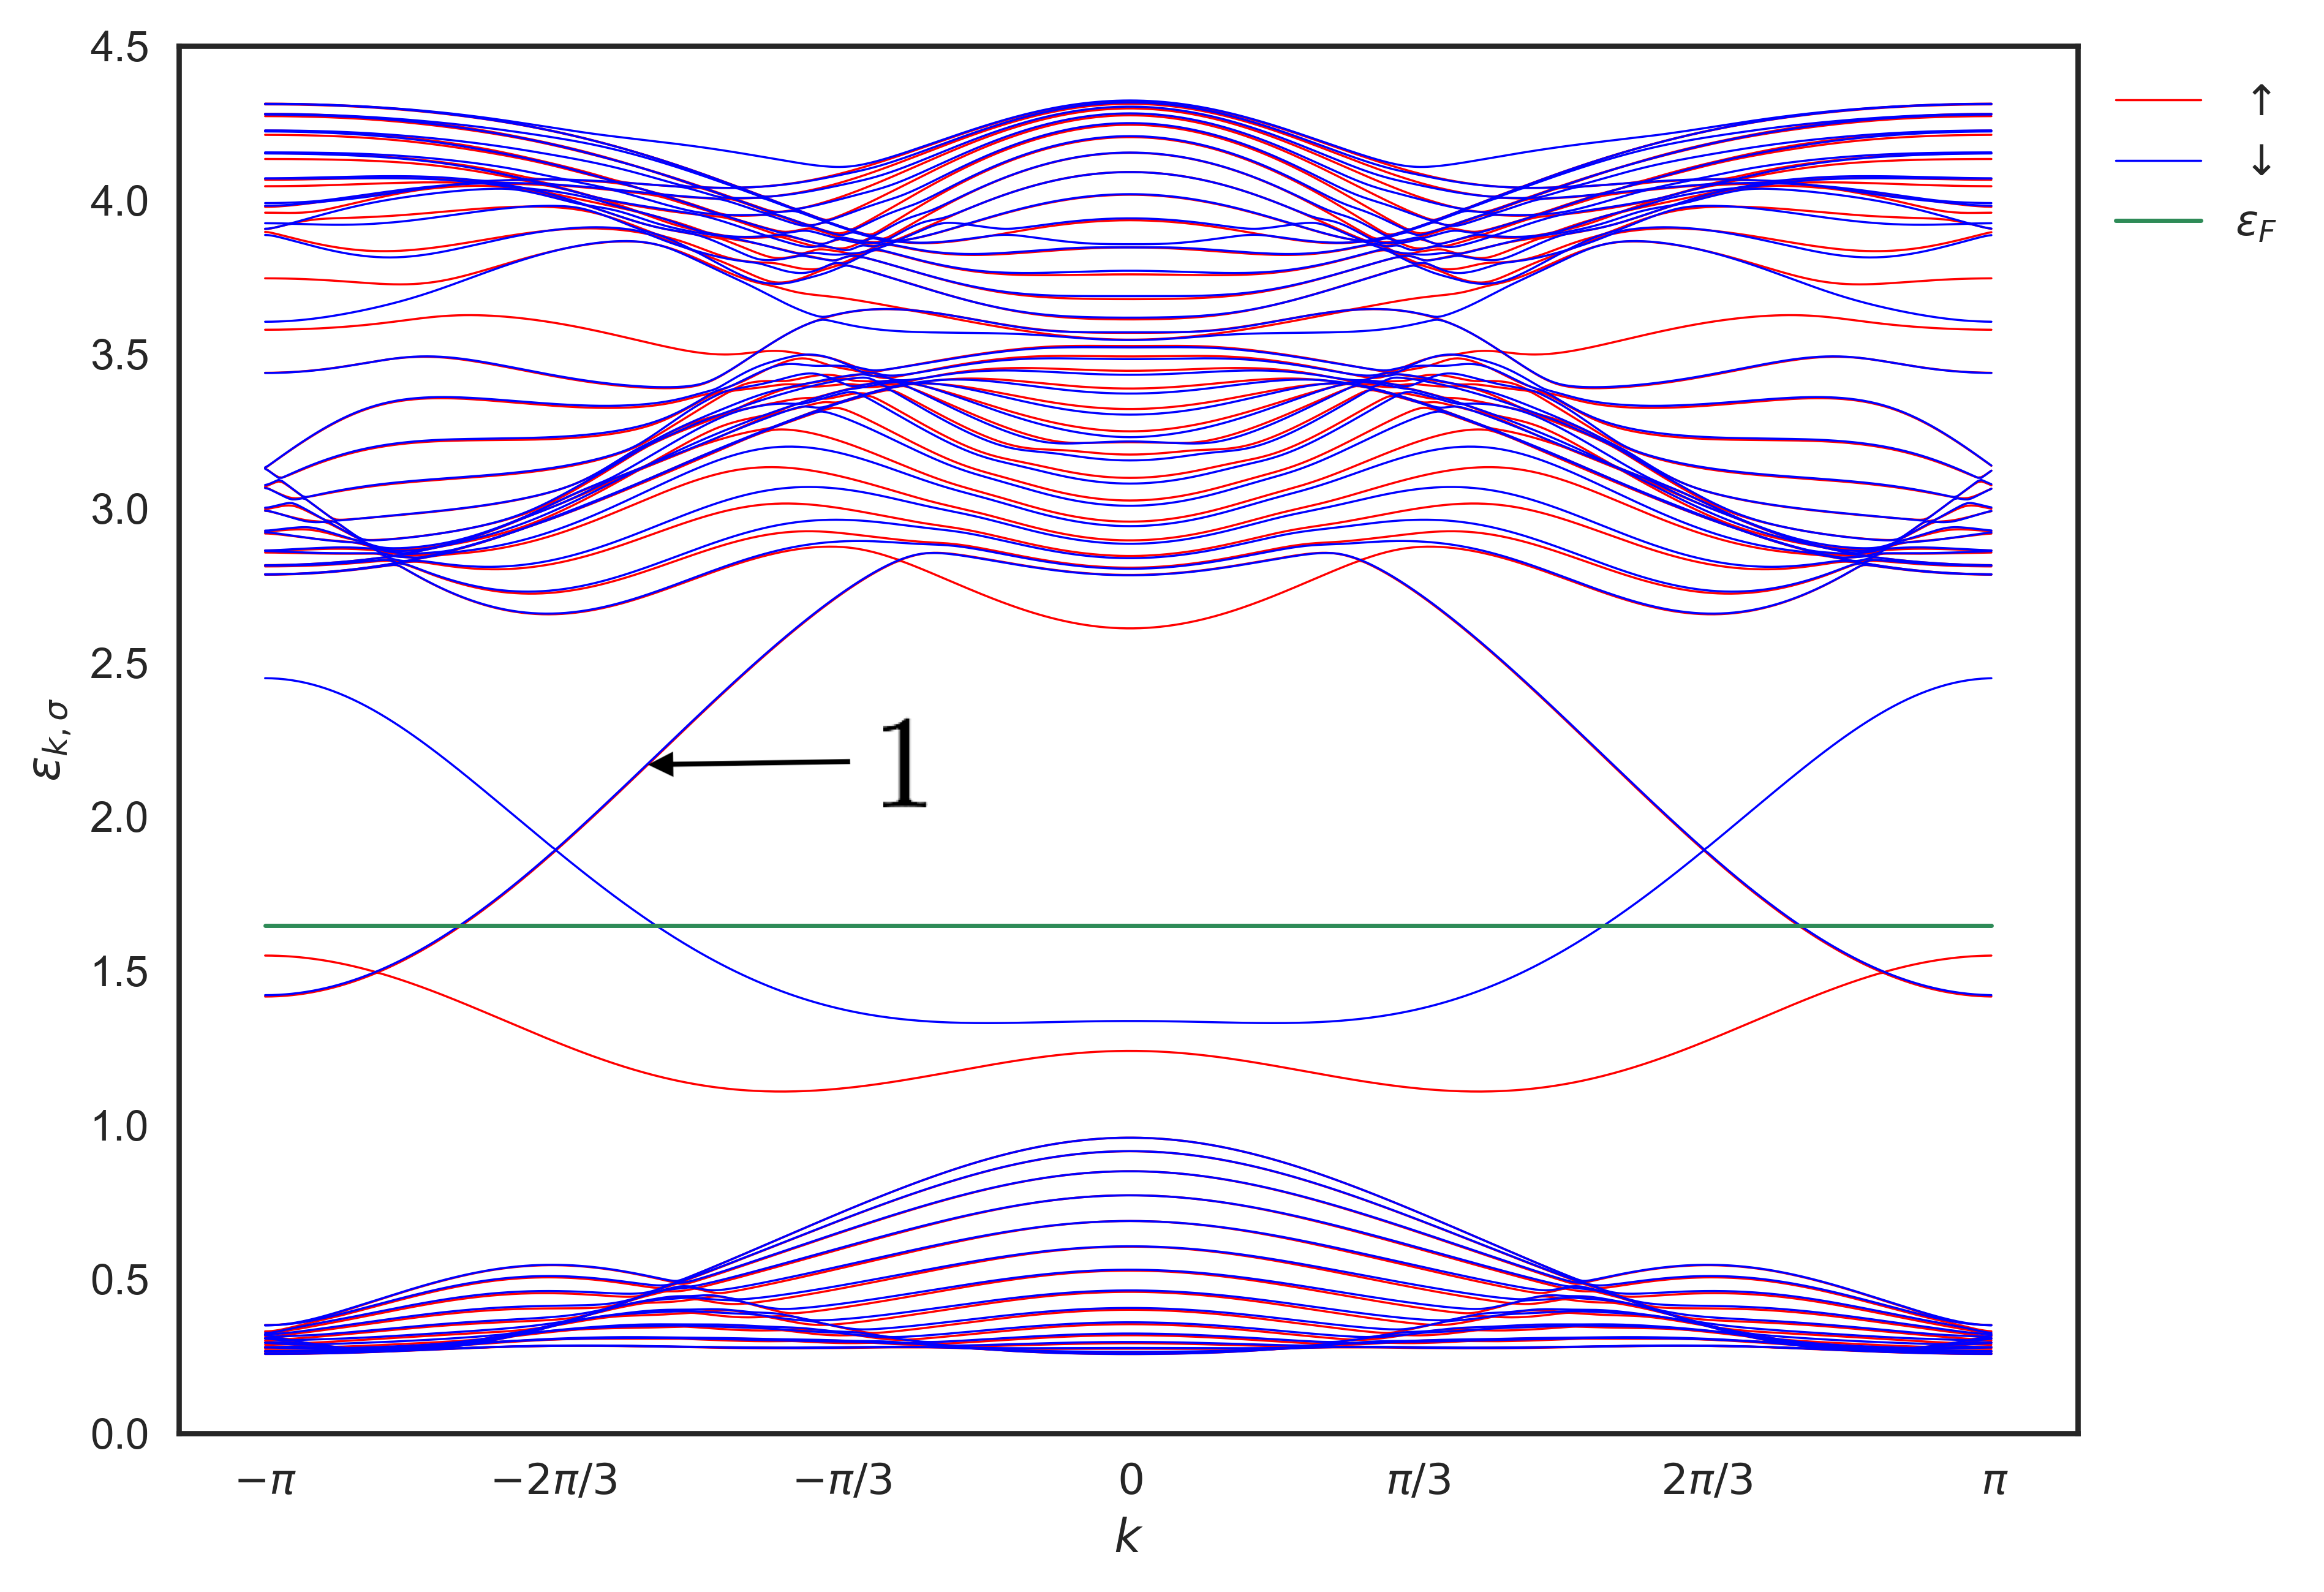
\includegraphics[width=6cm]{images/bands152.png}
  \caption{Comparison with \texttt{QUEST}}
  \label{fig:blade_flow_pressure}
\end{figure}

\begin{figure}[H]
  \centering
  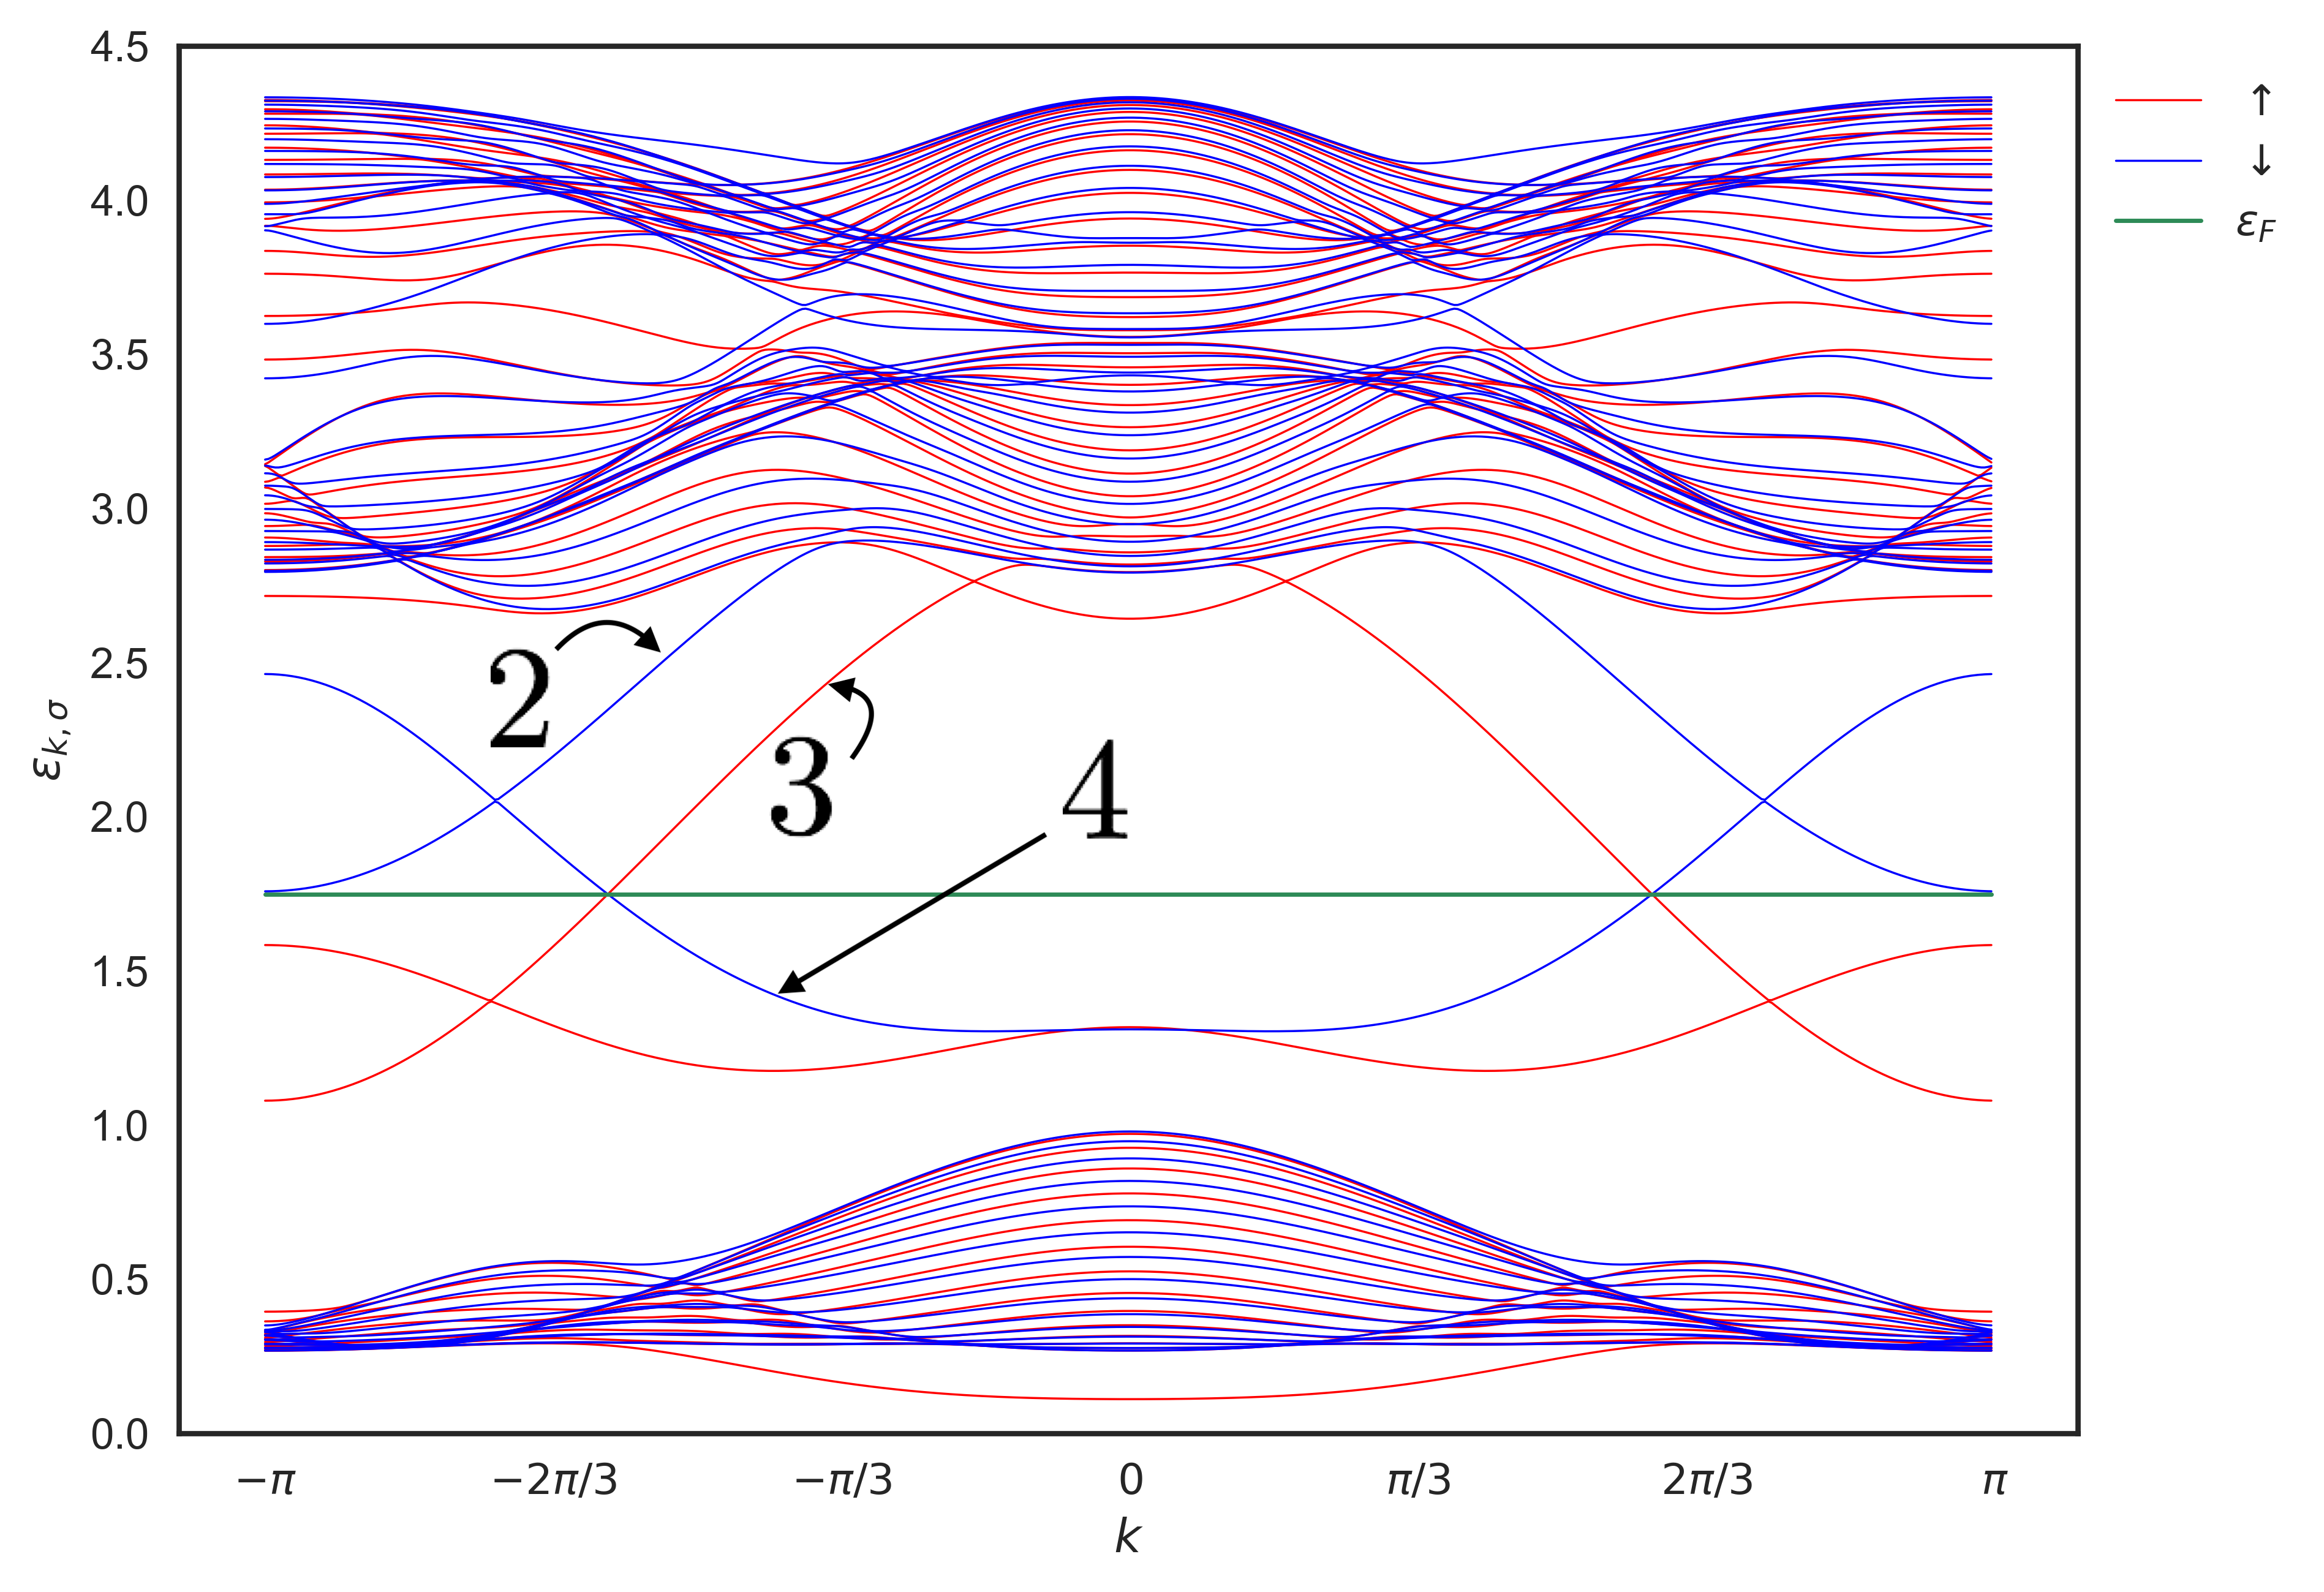
\includegraphics[width=6cm]{images/bands154.png}
  \caption{Comparison with \texttt{QUEST}}
  \label{fig:blade_flow_pressure}
\end{figure}

\begin{figure}[H]
  \centering
  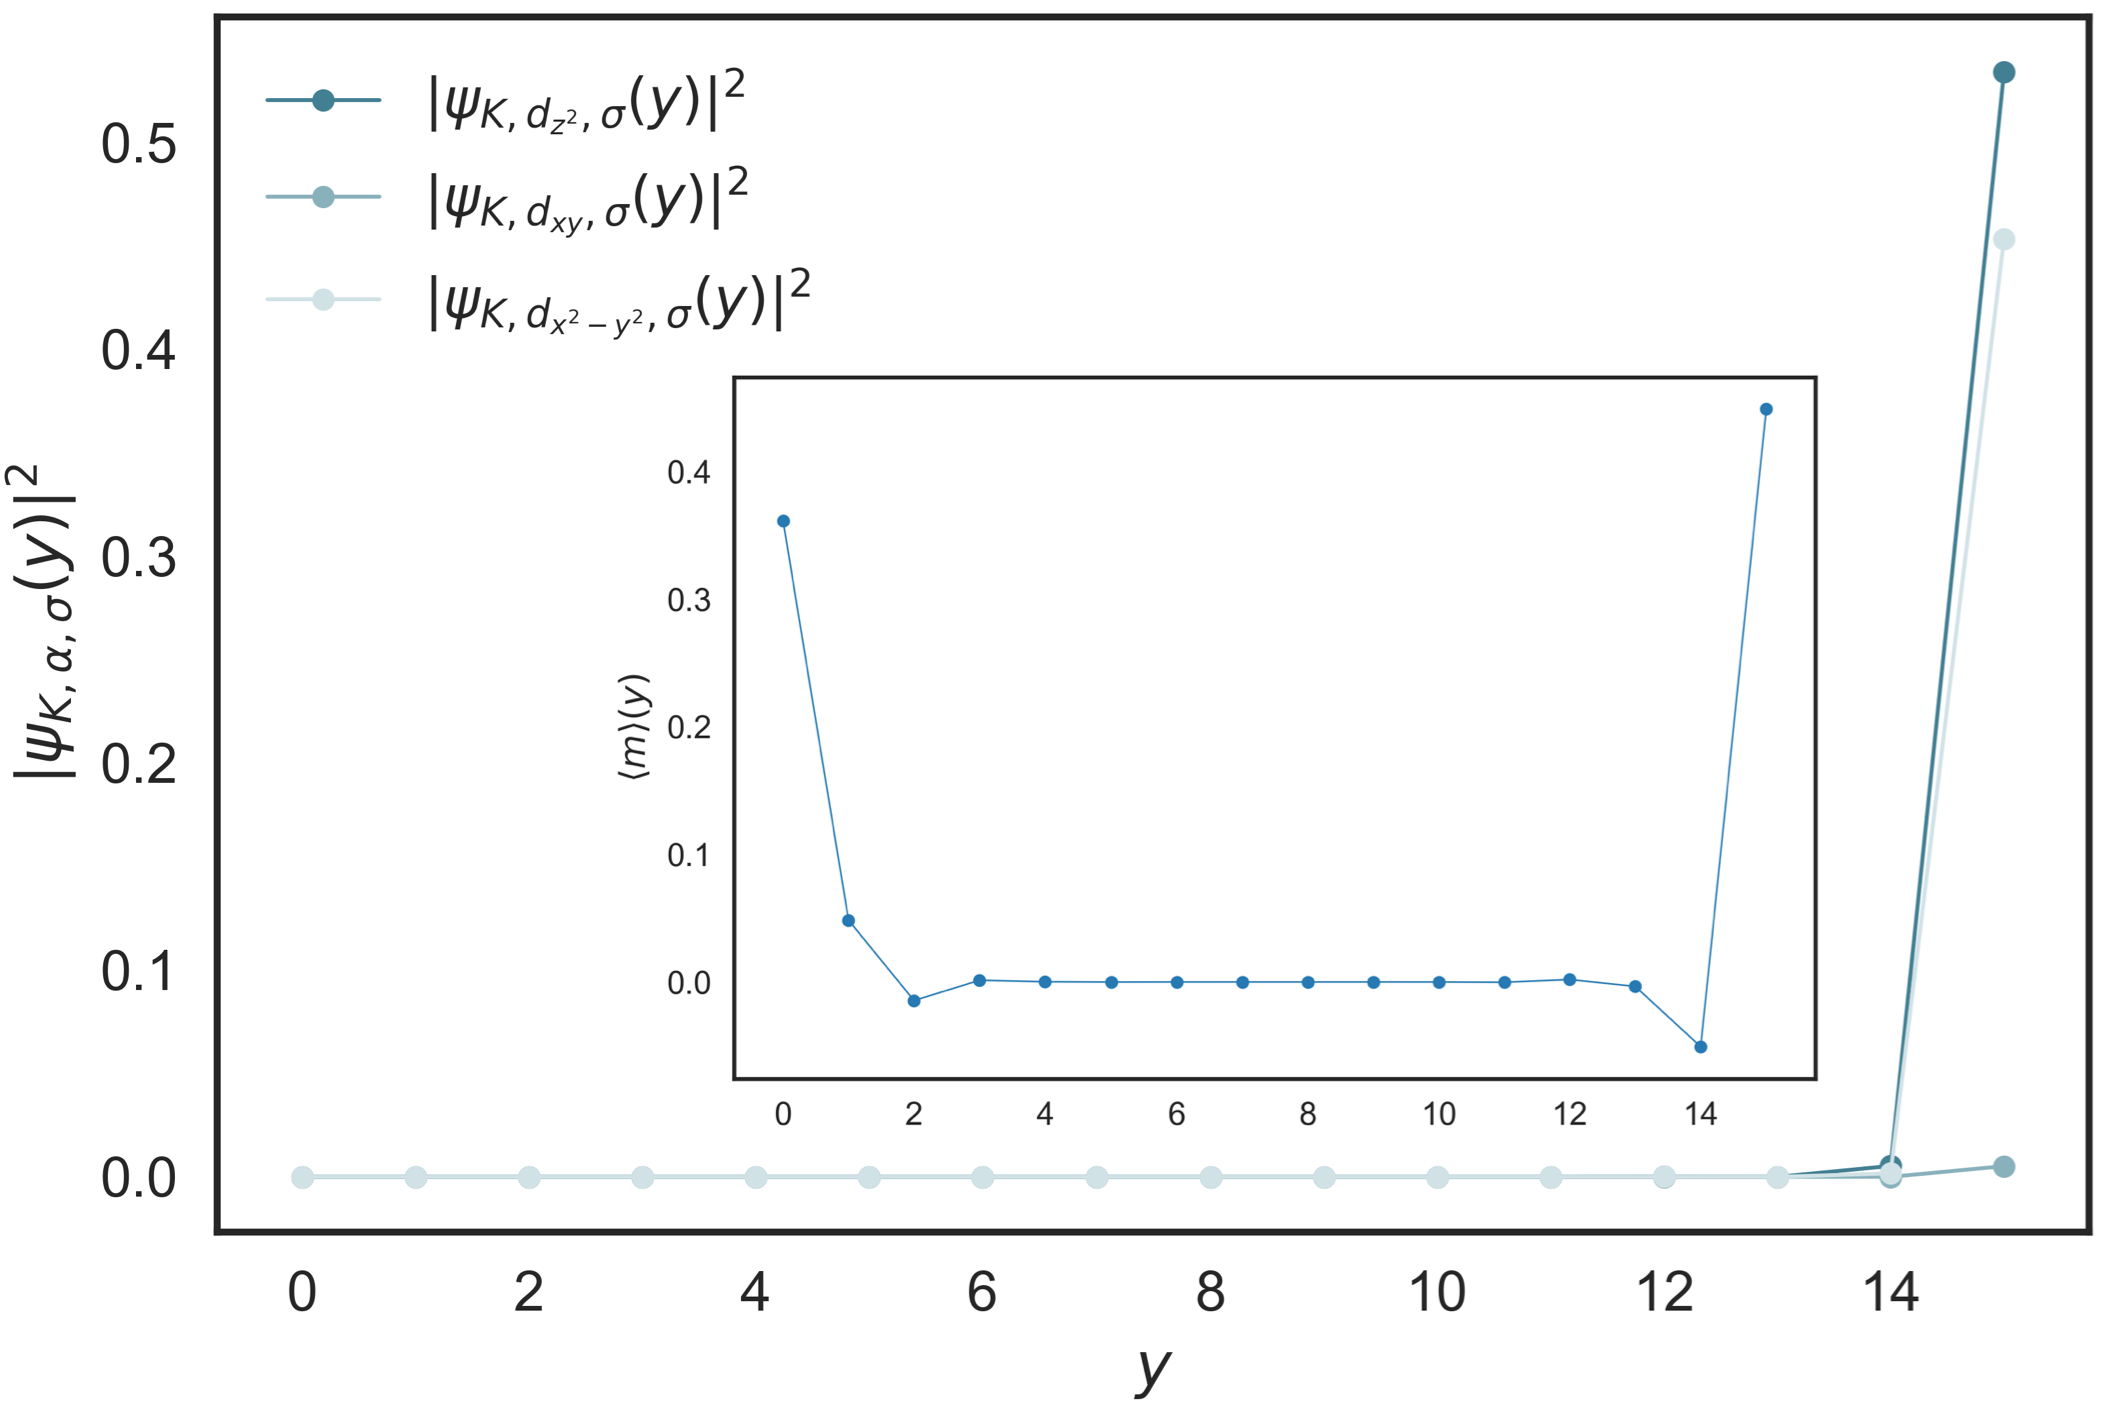
\includegraphics[width=6cm]{images/bottomEdgeMagProfU154.png}
  \caption{Comparison with \texttt{QUEST}}
  \label{fig:blade_flow_pressure}
\end{figure}

\begin{figure}[H]
  \centering
  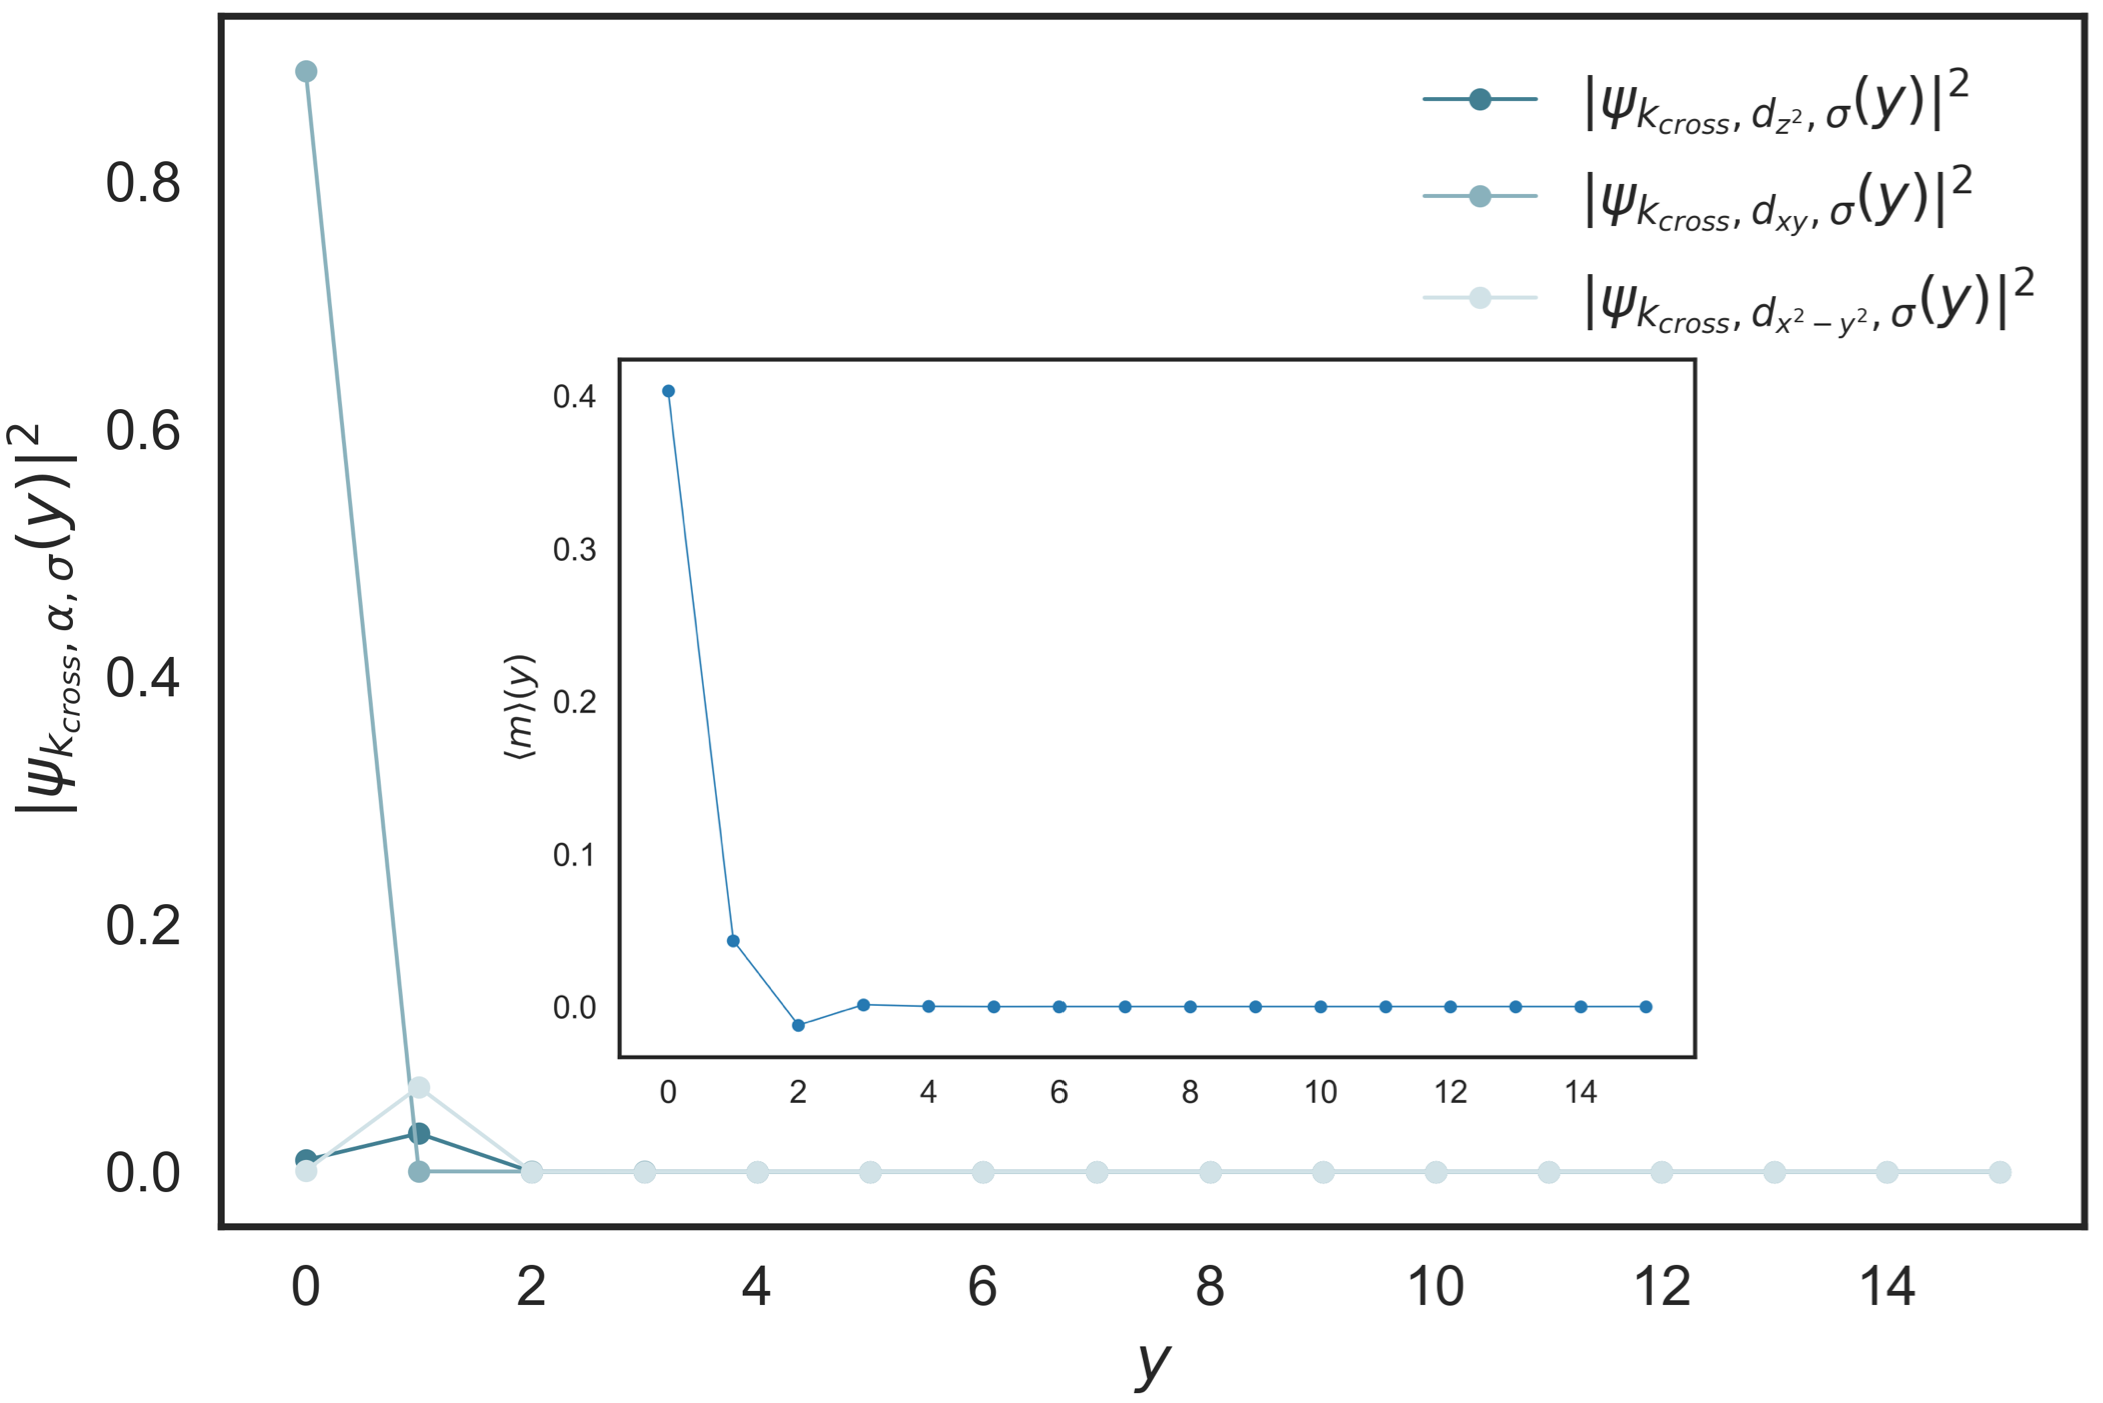
\includegraphics[width=6cm]{images/topEdgeMagProfU13.png}
  \caption{Comparison with \texttt{QUEST}}
  \label{fig:blade_flow_pressure}
\end{figure}

\begin{figure}[H]
  \centering
  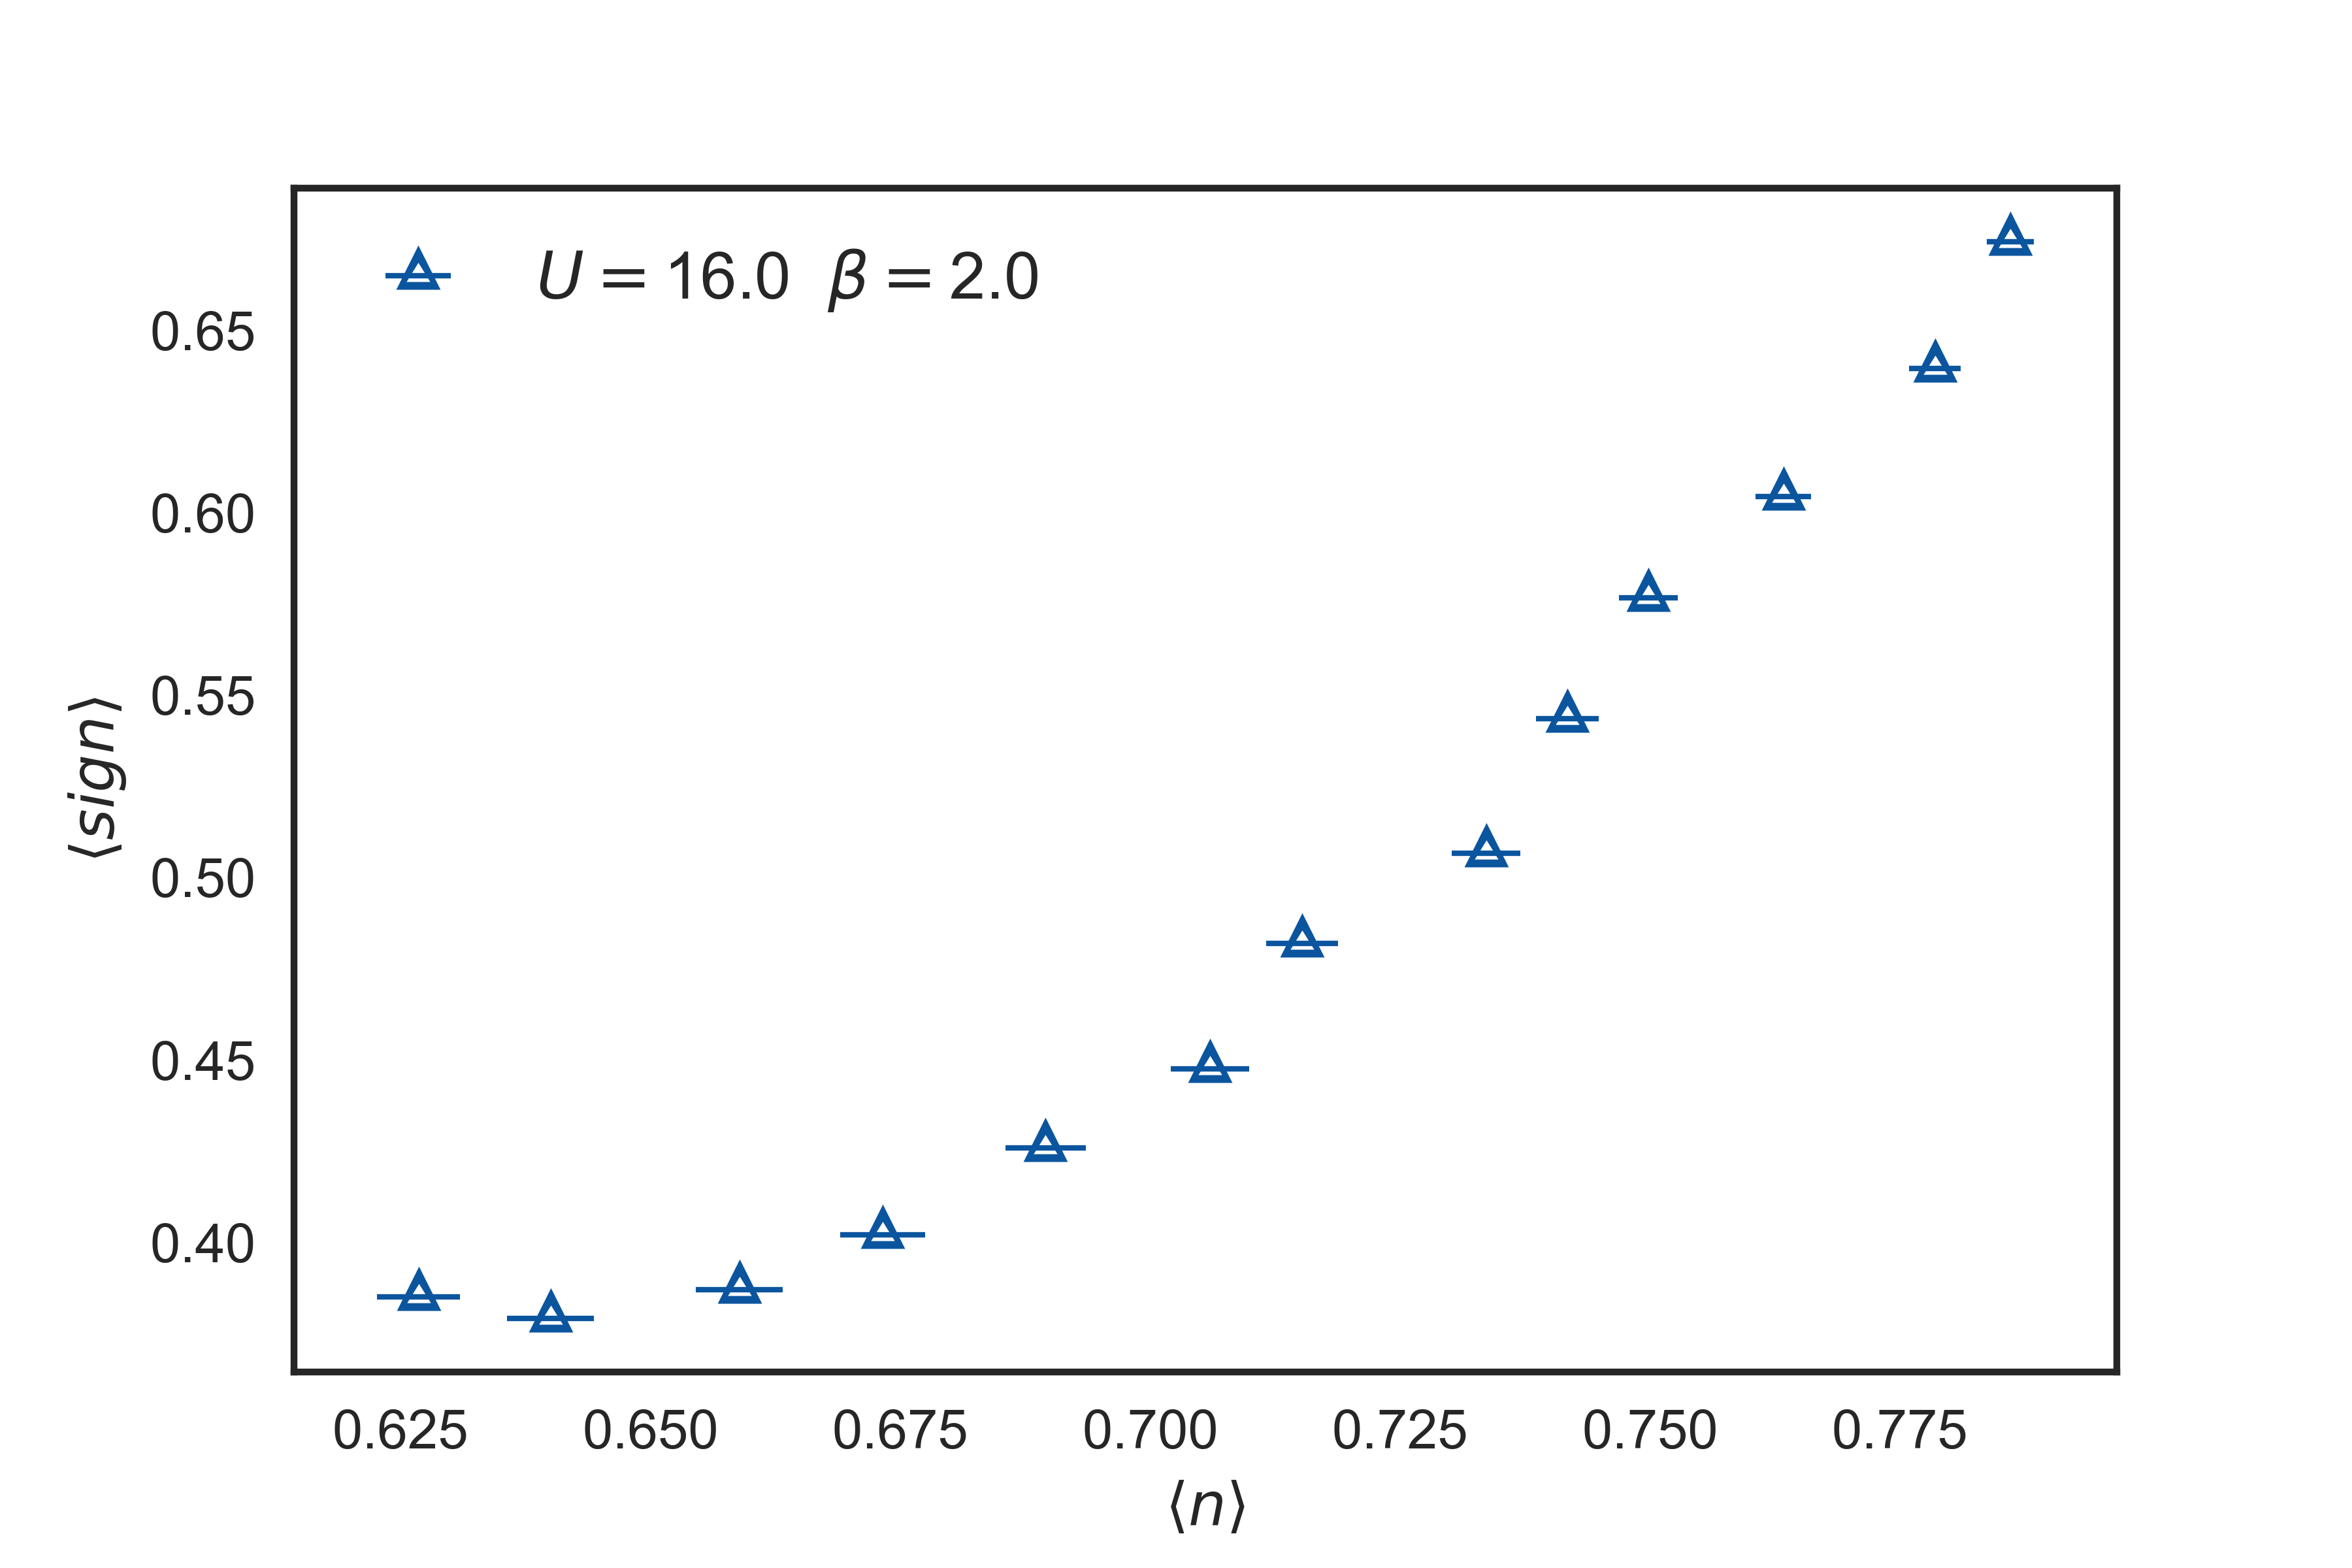
\includegraphics[width=6cm]{images/signTMDdensSignU16beta2.png}
  \caption{Comparison with \texttt{QUEST}}
  \label{fig:blade_flow_pressure}
\end{figure}

\begin{figure}[H]
  \centering
  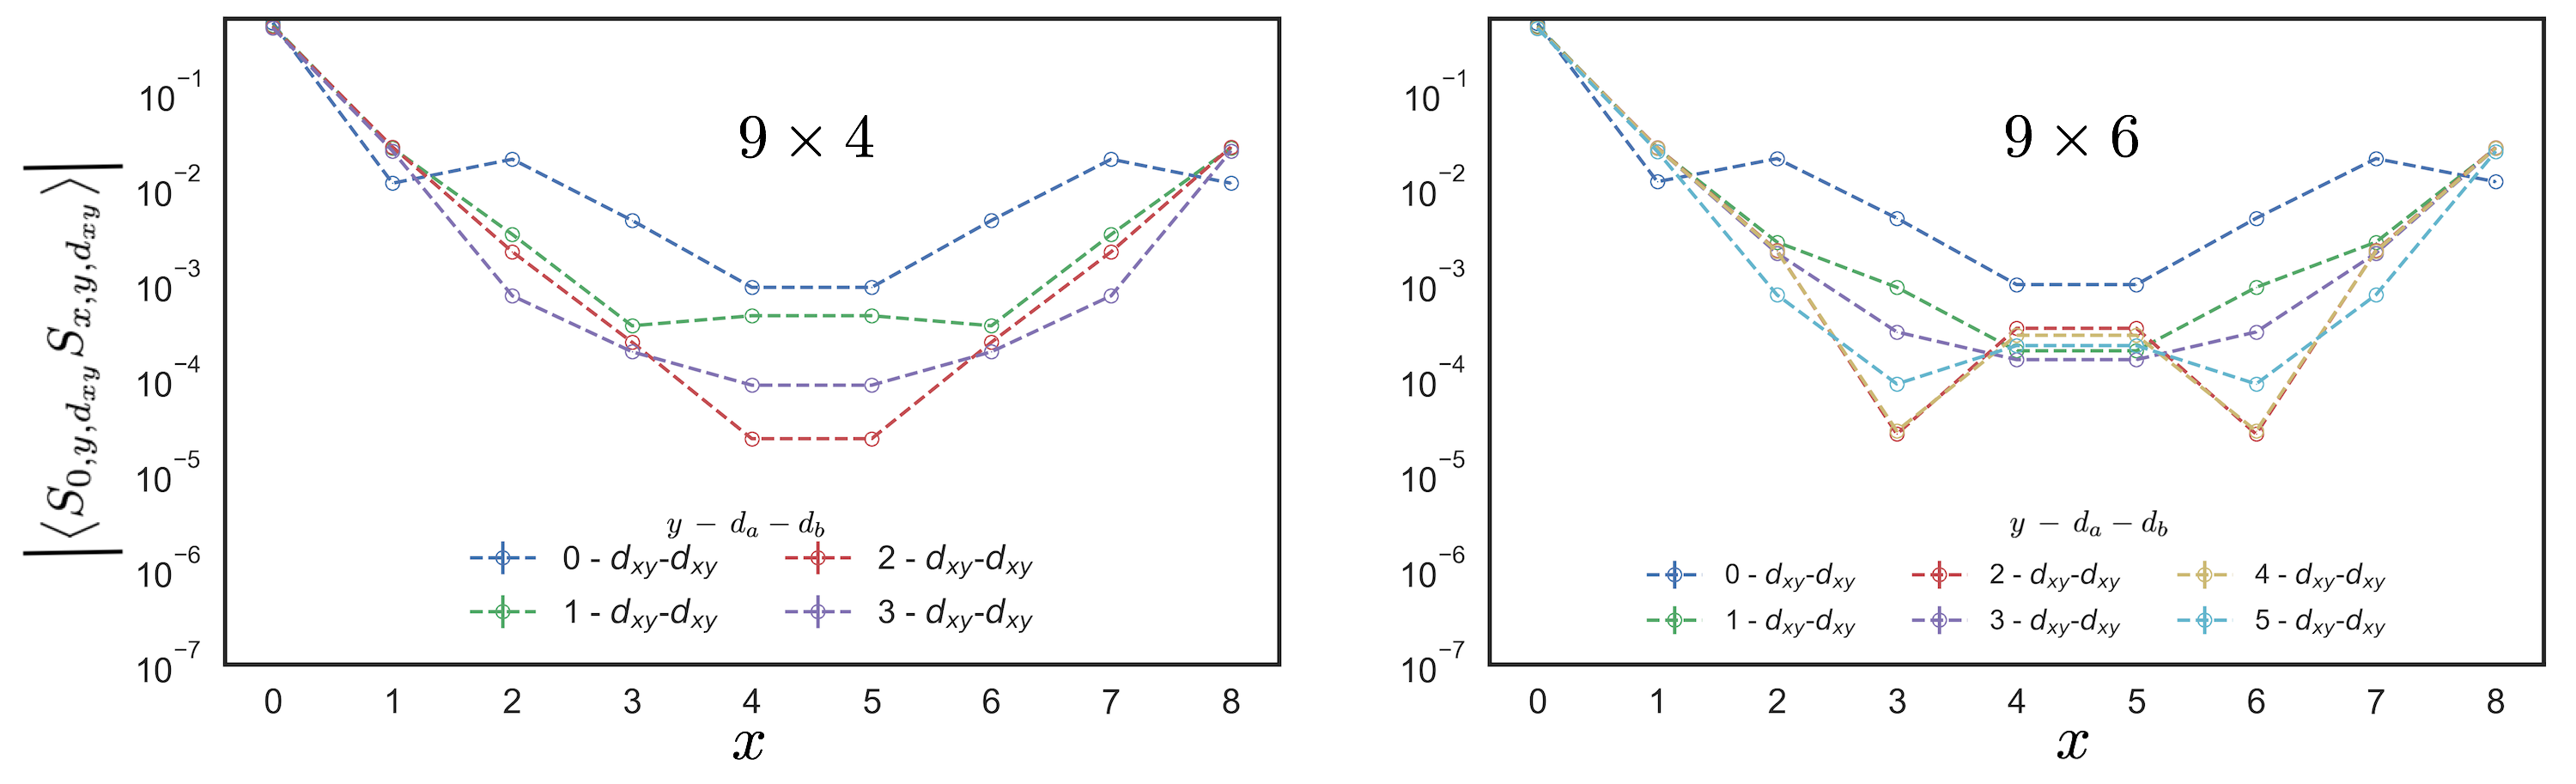
\includegraphics[width=6cm]{images/tmdFinalxyxy.png}
  \caption{Comparison with \texttt{QUEST}}
  \label{fig:blade_flow_pressure}
\end{figure}

\begin{figure}[H]
  \centering
  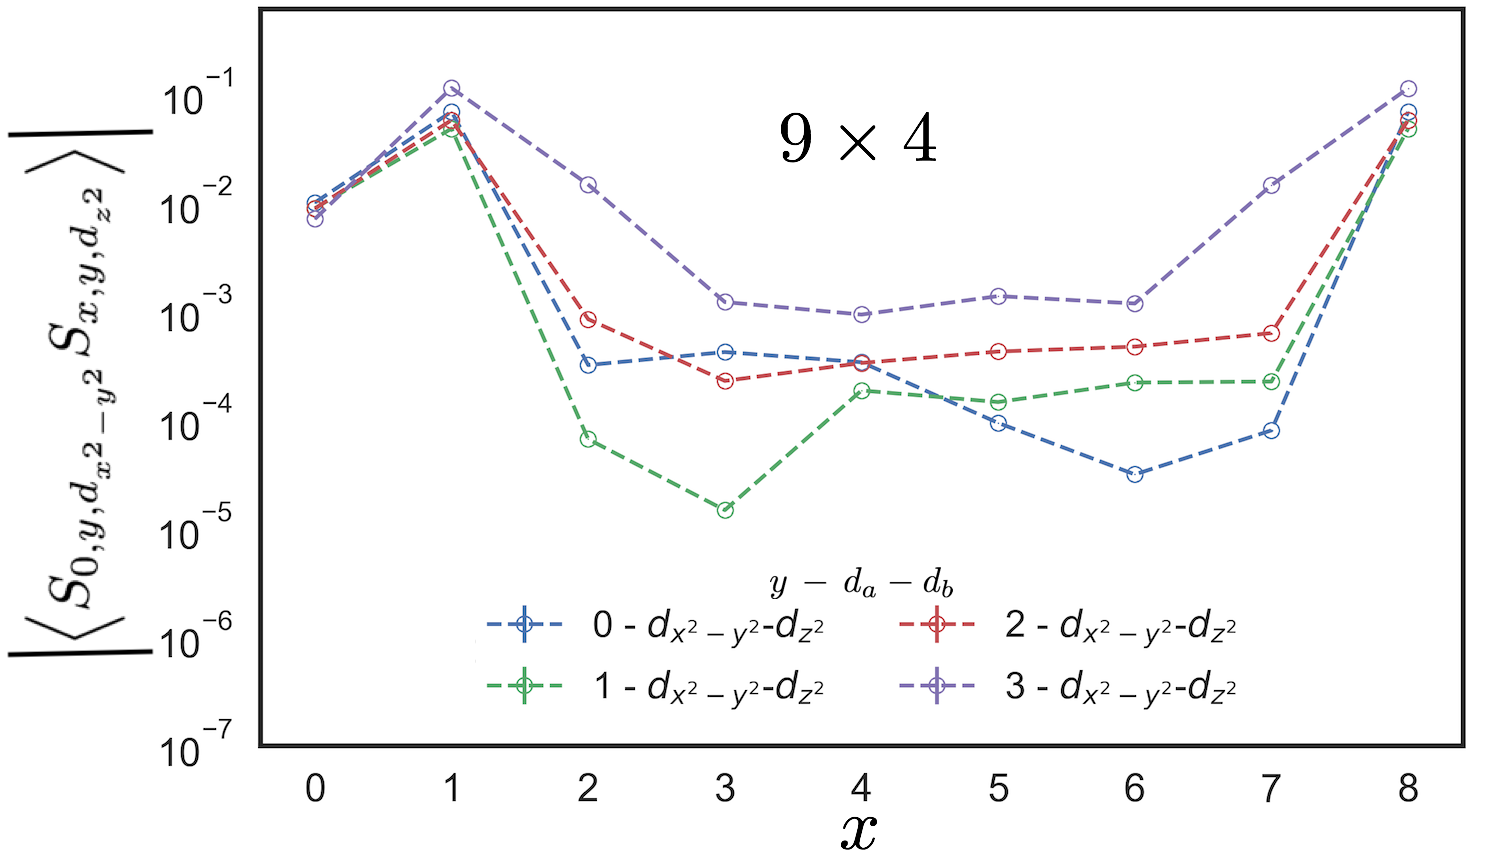
\includegraphics[width=6cm]{images/tmdFinalx2y2z2.png}
  \caption{Comparison with \texttt{QUEST}}
  \label{fig:blade_flow_pressure}
\end{figure}

\begin{figure}[H]
  \centering
  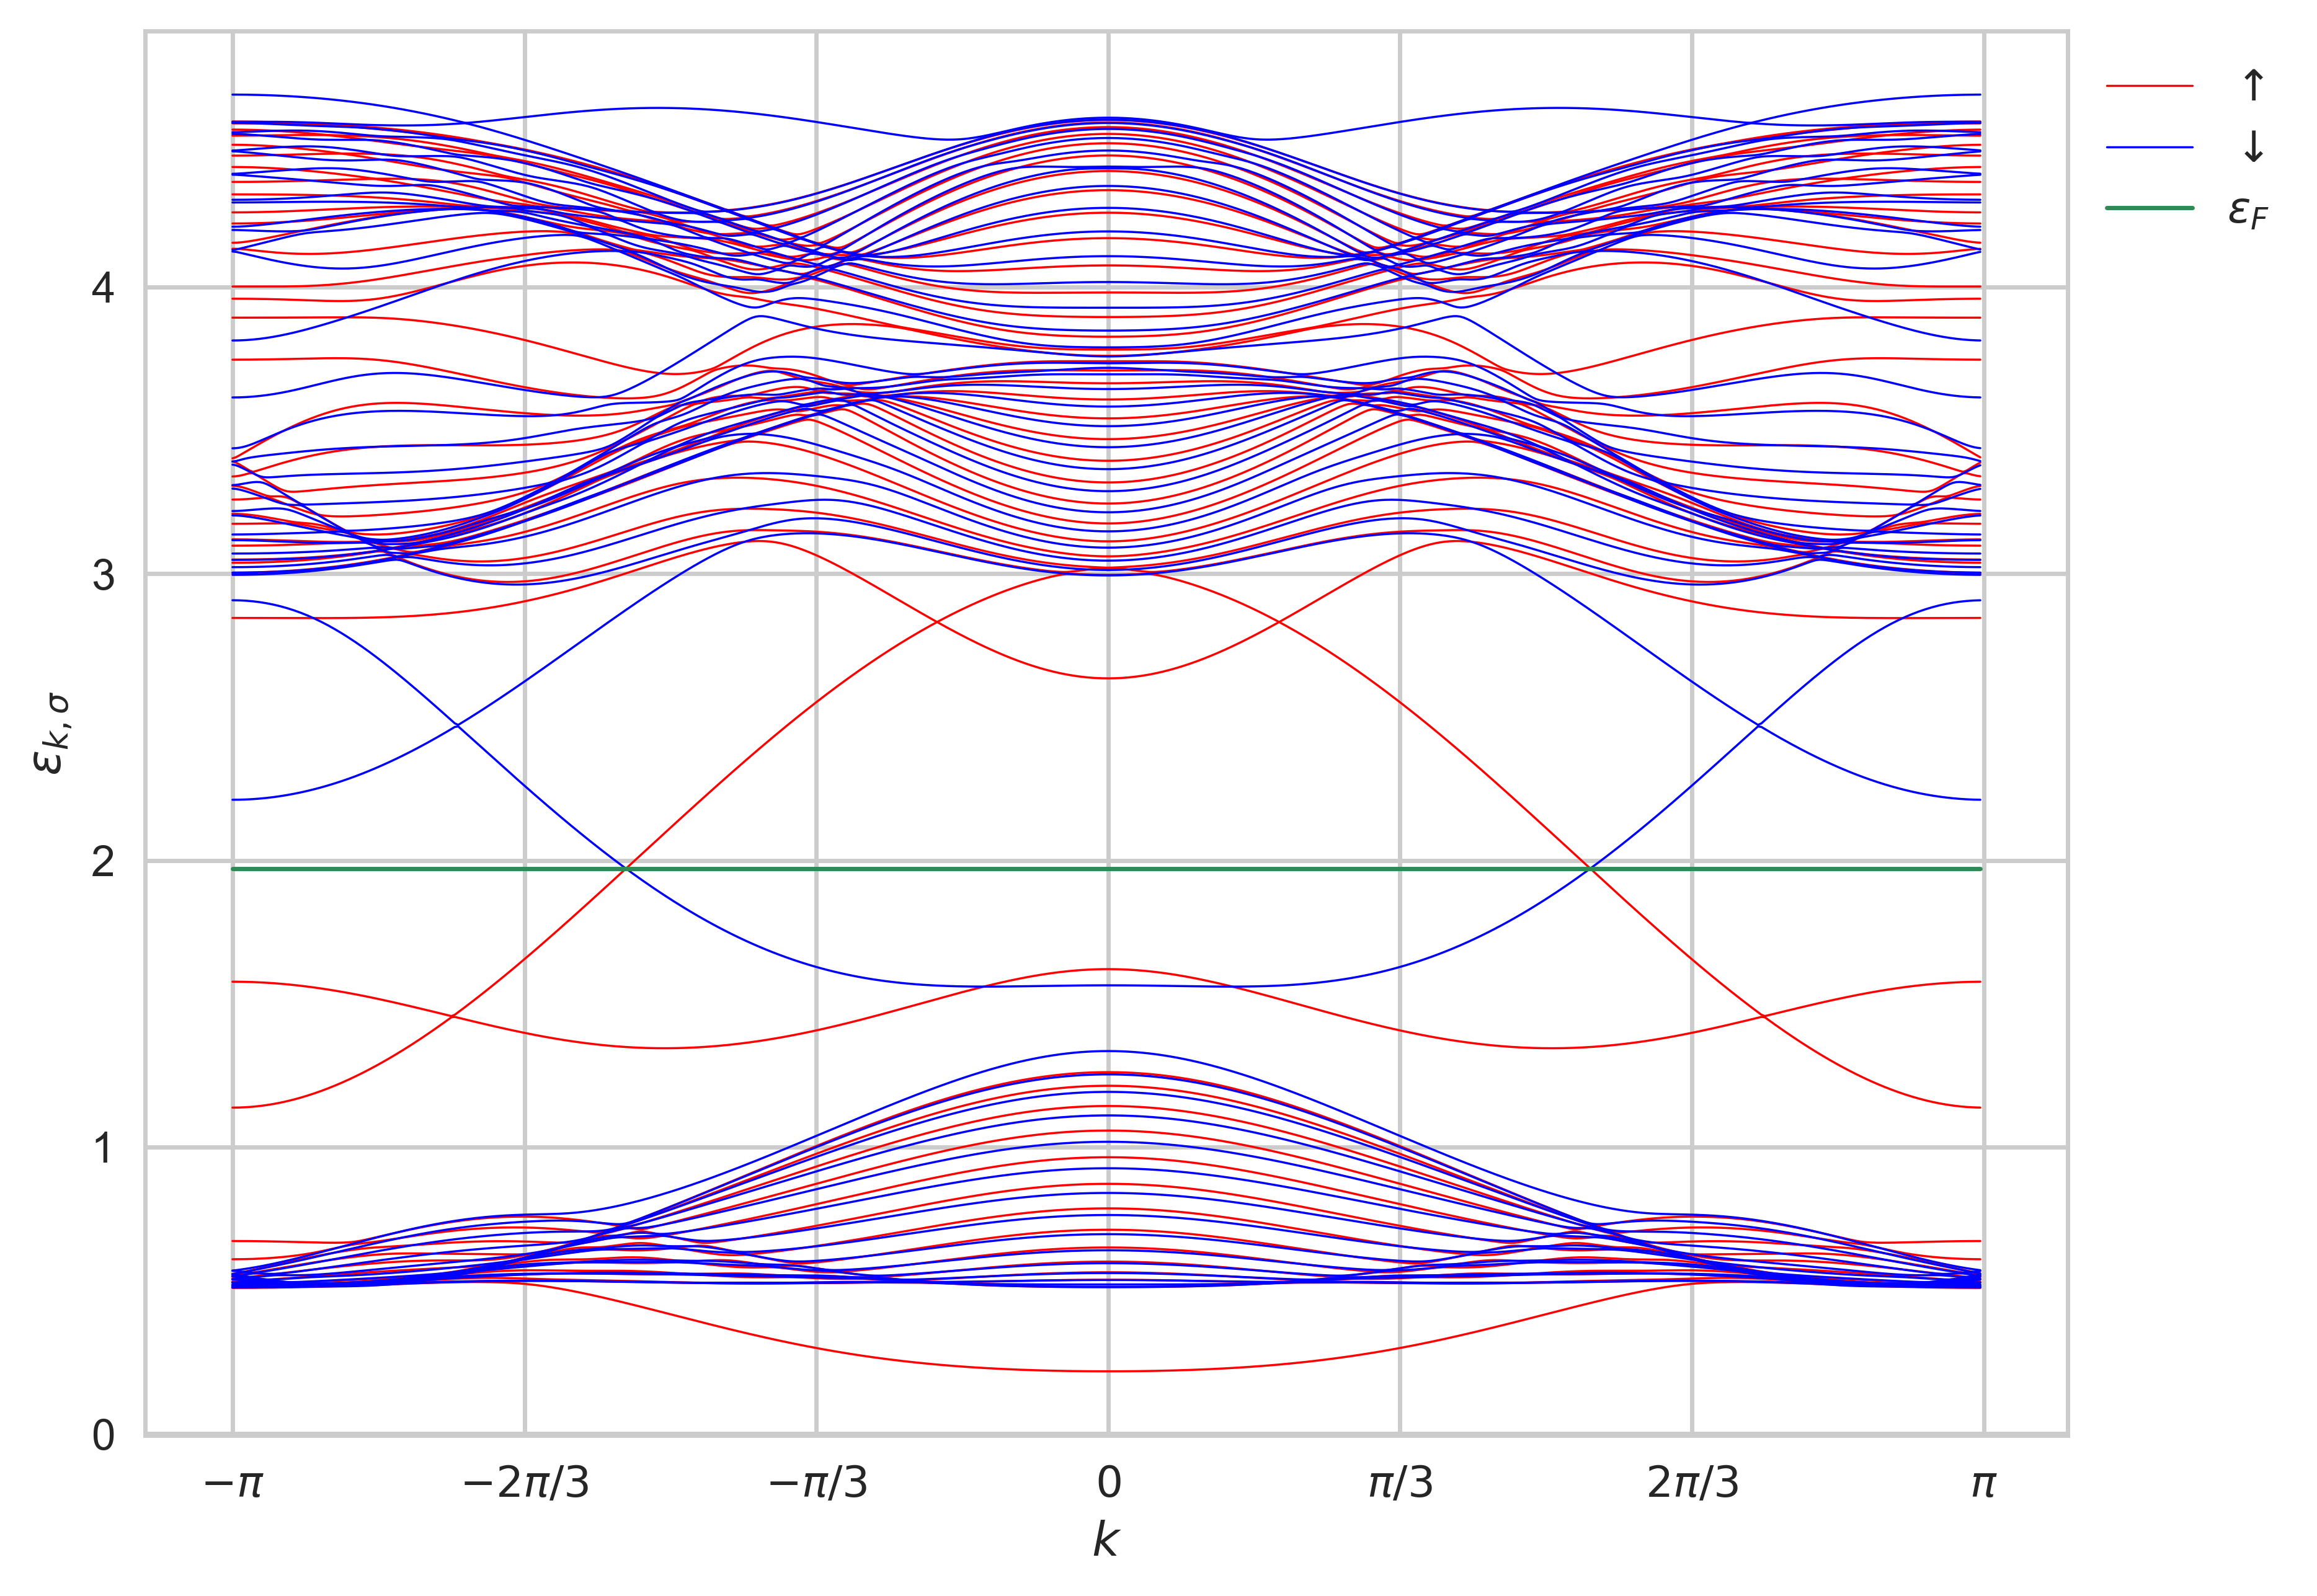
\includegraphics[width=6cm]{images/bands_Nx=512.png}
  \caption{Comparison with \texttt{QUEST}}
  \label{fig:blade_flow_pressure}
\end{figure}

%As seen in Fig.\ref{fig:blade_flow_pressure}...


%%%%%%%%%%%%%%%%%%%%%%%%%%%%%%%%%%%%%%%%%%%%%%%%%%%%%%%%%%%%%%%%%%%%%%
%\subsection{Sub-section...}

%More text...

%Table~\ref{table:simple} summarizes...

%\begin{table}[!h]
%  \begin{center}
%    \begin{tabular}{lccc}
%      Model           & $C_L$ & $C_D$ & $C_{M y}$ \\
%      \hline
%      Euler           & 0.083 & 0.021 & -0.110    \\
%      Navier--Stokes  & 0.078 & 0.023 & -0.101    \\
%      \hline
%    \end{tabular}
%  \end{center}
%  \caption[Table caption shown in TOC]{Table caption}
%  \label{table:simple}
%\end{table}

%As seen in Tab.\ref{table:simple}...

